\section*{第一章 平面向量}

\section*{一、向量的概念和线性运算}

\section*{【典型例题和解题技巧】}

1. 向量的概念.

(1)既有大小又有方向的量,称为向量,常用 $\vv{a},\vv{AB}$ 表示. 向量的大小称为向量的模,用 $\left| \vv{a}\right|$ 表示. 特别的,模为 0 的向量称为零向量,零向量的方向任意. 模长为 1 的向量称为单位向量,与非零向量 $a$ 同向的单位向量是 $\dfrac{\vv{a}}{\left| \vv{a}\right| }$ .

(2)方向相同、模相等的向量称为相等的向量；方向相反,模相等的两个向量互为负向量. 方向相同或相反的两个向量为平行向量.

例 1 判断下列各命题是否正确:

(1)零向量没有方向；(2)若 $\left| \vv{a}\right|  = \left| \vv{b}\right|$ ,则 $\vv{a} = \vv{b}$ ；(3)单位向量都相等；

(4)两相等向量若共起点,则终点也相同；(5)若 $a = b,b = c$ ,则 $a = c$ ；

(6)若 $\vv{a}//\vv{b},\vv{b}//\vv{c}$ ,则 $\vv{a}//\vv{c}$ ；(7) $\vv{a} = \vv{b}$ 的充要条件是 $\left| \vv{a}\right|  = \left| \vv{b}\right|$ 且 $\vv{a}//\vv{b}$ .

解(1)不正确,零向量方向任意. (2)不正确,条件说明模相等,方向可以不相同.

(3)不正确,单位向量的模为 1,方向很多. (4)正确. (5)正确,向量相等有传递性.

(6)不正确,因若 $b = 0$ ,则不共线的向量 $a,c$ 也有 $a//0,0//c$ .

(7)不正确,当 $\vv{a}//\vv{b}$ ,且方向相反时,即使 $\left| \vv{a}\right|  = \left| \vv{b}\right|$ ,也不能得到 $\vv{a} = \vv{b}$ .

2. 向量的线性运算:加法、减法、数乘.

(1)向量的加法:求两个向量和的运算叫做向量的加法. 设 $\vv{AB} = \vv{a},\vv{BC} = \vv{b}$ ,则 $\vv{a} + \vv{b} = \vv{AB}$  $+ \vv{BC} = \vv{AC}$ . 向量的加法有“三角形法则”与“平行四边形法则”.

注:(1) $0 + a = a + 0 = a.$ (2)向量加法满足交换律与结合律.

(2)向量的减法:向量 $a$ 加上 $b$ 的负向量叫做 $a$ 与 $b$ 的差,记作: $a - b = a + \left( {-b}\right)$ . 求两个向量差的运算,叫做向量的减法. $a - b$ 可以表示为从 $b$ 的终点指向 $a$ 的终点的向量 $(a,b$ 有共同起点).

(3)实数与向量的积:实数 $\lambda$ 与向量 $\vv{a}$ 的积是一个向量,记作 $\lambda \vv{a}$ ,它的长度与方向规定如下:(1) $\left| {\lambda a}\right|  = \left| \lambda \right|  \cdot  \left| a\right|$ ；(2)当 $\lambda  > 0$ 时, ${\lambda a}$ 的方向与 $a$ 的方向相同；当 $\lambda  < 0$ 时, ${\lambda a}$ 的方向与 $a$ 的方向相反；当 $\lambda  = 0$ 时, ${\lambda a} = 0$ ,方向是任意的. 数乘向量满足交换律、结合律与分配律.

例 2 如图 1 所示,已知正六边形 ${ABCDEF},O$ 是它的中心,若 $\vv{BA} = \vv{a},\vv{BC} = \vv{b}$ ,试用 $\vv{a},\vv{b}$ 将向量 $\vv{OE},\vv{BF},\vv{BD},\vv{FD}$ 表示出来.

解 因为六边形 ${ABCDEF}$ 是正六边形,所以它的中心 $O$ 及顶点 $A$ , $B,C$ 四点构成平行四边形 ${ABCO}$ ,所以 $\vv{BA} + \vv{BC} = \vv{BA} + \vv{AO} = \vv{BO}$ ,即 $\vv{BO} = \vv{a} + \vv{b}$ ,所以 $\vv{OE} = \vv{BO} = \vv{a} + \vv{b}$ ,由于 $A,B,O,F$ 四点也构成平行四边形 ${ABOF}$ ,所以 $\vv{BF} = \vv{BO} + \vv{OF} = \vv{BO} + \vv{BA} = \vv{a} + \vv{b} + \vv{a} = 2\vv{a} + \vv{b}$ ,同样在平行四边形 ${BCDO}$ 中, $\vv{BD} = \vv{BC} + \vv{CD} = \vv{BC} + \vv{BO} = \vv{b} + \left( {\vv{a} + \vv{b}}\right)  = \vv{a} + 2\vv{b}$ , $\vv{FD} = \vv{BC} - \vv{BA} = \vv{b} - \vv{a}.$

\begin{center}
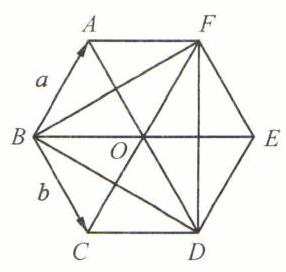
\includegraphics[width=0.2\textwidth]{bodyxb/src/bo_d20aucref24c73anc48g_3_1175_122_286_272_0.jpg}
\end{center}


(图 1)

例 $3{e}_{1},{e}_{2}$ 是不共线的向量,已知向量 $\vv{AB} = 2{e}_{1} + k{e}_{2},\vv{CB} = {e}_{1} + 3{e}_{2},\vv{CD} = 2{e}_{1} - {e}_{2}$ ,若 $A,B,D$ 三点共线,求 $k$ 的值.

解 $\vv{BD} = \vv{CD} - \vv{CB} = {\vv{e}}_{1} - 4{\vv{e}}_{2}$ ,设 $\vv{AB} = \lambda \vv{BD},\therefore 2{\vv{e}}_{1} + k{\vv{e}}_{2} = \lambda \left( {{\vv{e}}_{1} - 4{\vv{e}}_{2}}\right)$ ,

得 $\lambda  = 2,k =  - {4\lambda } \Rightarrow  k =  - 8$ . 【训练题】 (A)

1. 下列物理量:①质量,②速度,③位移,④力,⑤加速度,③路程,改密度,运动,其中不是向量的有(D)

(A) 1 个. (B) 2 个. (C) 3 个. (D) 4 个.

2. 给出下列命题 ①若 $a = b,b = c$ ,则 $a = c$ ； ${\Delta a} = b$ 的充要条件是 $\left| a\right|  = \left| b\right|$ 且 $a//b$ ；若 $a//$  $b,b//c$ ,则 $a//c$ . 其中正确命题的个数为 (   )

(A) 0 个. (B) 1 个.

(C) 2 个. (D) 3 个.

设 $D,E,F$ 分别为 $\bigtriangleup {ABC}$ 的三边 ${BC},{CA},{AB}$ 的中点,则 $\vv{EB} + \vv{FC} =$ ( $C$ ) (A) $\vv{BC}$ . (B) $\dfrac{1}{2}\vv{AD}$ .

(C) $\vv{AD}$ . (D) $\dfrac{1}{2}\vv{BC}$ . $= \dfrac{1}{2}\left( {\vv{AB} + \vv{AC}}\right)$  $= \vv{AD}$

4. 如图, $D,E,F$ 分别为 $\bigtriangleup {ABC}$ 的三边 ${AB},{BC},{CA}$ 的中点,则 ( $A$ )

\begin{center}
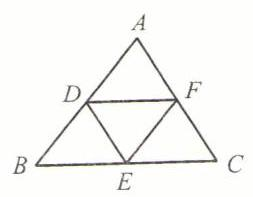
\includegraphics[width=0.2\textwidth]{bodyxb/src/bo_d20aucref24c73anc48g_3_1208_1565_253_197_0.jpg}
\end{center}


(第 4 题)

(A) $\vv{AD} + \vv{BE} + \vv{CF} = \vv{0}$ . (B) $\vv{BD} - \vv{CF} + \vv{DF} = \vv{0}$ .

(C) $\vv{AD} + \vv{CE} - \vv{CF} = \vv{0}$ . (D) $\vv{BD} - \vv{BE} - \vv{FC} = \vv{0}$ .

5 设 $D,E,F$ 分别是 $\bigtriangleup {ABC}$ 的三边 ${BC},{CA},{AB}$ 上的点,且 $\vv{DC} = 2\vv{BD}$ , $\vv{CE} = 2\vv{EA},\vv{AF} = 2\vv{FB}$ ,则 $\vv{AD} + \vv{BE} + \vv{CF}$ 与 $\vv{BC}$ (C) (A) 方向相同, 模长相等. (B) 方向相同, 模长不相等. (C) 方向相反, 模长相等. (D) 方向相反, 模长不相等.


⑥ 已知 $O,A,B$ 是平面上的三个点,直线 ${AB}$ 上有一点 $C$ ,满足 $2\vv{AC} + \vv{CB} = \vv{0}$ ,则 $\vv{OC} = \left( \text{ A }\right)$ (A) $2\vv{OA} - \vv{OB}$ . (B) $- \vv{OA} + 2\vv{OB}$ .

(C) $\dfrac{2}{3}\vv{OA} - \dfrac{1}{3}\vv{OB}$ . (D) $- \dfrac{1}{3}\vv{OA} + \dfrac{2}{3}\vv{OB}$ . 平面向量 $\vv{a},\vv{b}$ 共线的充要条件是 ( 奘 (A) $a,b$ 方向相同. (B) $a,b$ 两向量中至少有一个为零向量. (C) 存在 $\lambda  \in  \mathbf{R}$ ,使得 $\vv{b} = \lambda \vv{a}$ . (D) 存在不全为零的实数 ${\lambda }_{1},{\lambda }_{2}$ ,使得 ${\lambda }_{1}\vv{a} + {\lambda }_{2}\vv{b} = \vv{0}$ . 8 设 $a,b$ 都是非零向量,下列四个条件中,使 $\dfrac{a}{\left| a\right| } = \dfrac{b}{\left| b\right| }$ 成立的充分条件是 (A) $\vv{a} =  - \vv{b}$ . (B) $\vv{a}//\vv{b}$ . (C) $\vv{a} = 2\vv{b}$ . (D) $\vv{a}//\vv{b}$ 且 $\left| \vv{a}\right|  = \left| \vv{b}\right|$ . ⑨ 已知 $G$ 是 $\bigtriangleup {ABC}$ 的重心,计算 $\vv{GA} + \vv{GB} + \vv{GC} = \vv{0}$ . 10. 在平行四边形 ${ABCD}$ 中,对角线 ${AC}$ 与 ${BD}$ 交于点 $O,\vv{AB} + \vv{AD} = \lambda \vv{AO}$ ,则 $\lambda  = 2$ . 11. 已知菱形 ${ABCD}$ 的边长是 2,则 $\left| {\vv{AB} - \vv{CB} + \vv{CD}}\right|  = 2$ . 12 若 $\vv{{P}_{1}P} =  - \dfrac{3}{4}\vv{P{P}_{2}}$ ,则下列各式:① $\vv{{P}_{2}{P}_{1}} = \dfrac{1}{3}\vv{{P}_{1}P}$ ；② $\vv{{P}_{2}P} = \dfrac{4}{3}\vv{{P}_{1}P}$ ；② $\vv{{P}_{1}P} =  - 3\vv{{P}_{1}{P}_{2}}$ ；


23. $\sqrt{P{P}_{2}} = 4\vv{{P}_{2}{P}_{1}}$ 中正确的是② ③ ① 填序号). $\vv{AD} = \vv{AB} + \vv{BD}$ 13 已知在 $\bigtriangleup {ABC}$ 中, $D$ 是 ${BC}$ 上的一点,且 $\vv{BD} = \lambda \vv{DC}$ ,求证: $\vv{AD} = \dfrac{\vv{AB} + \lambda \vv{AC}}{1 + \lambda }$ . $= \vv{AB} + \dfrac{\lambda \vv{BC}}{\lambda  + 1}$  $\vv{BA} = 2\vv{CB}$  $= \vv{AB} + \dfrac{\pi }{a + 1}\left( {\vv{AC} - \vv{AB}}\right)$ 15 设点 $O$ 在 $\bigtriangleup {ABC}$ 的内部,且有 $\vv{OA} + 2\vv{OB} + 3\vv{OC} = \vv{0}$ ,求 $\bigtriangleup {ABC}$ 的面积与 $\bigtriangleup {AOC}$ 的面积设 $\dfrac{S\Delta ABC}{S\Delta AOC} = 3$  $\vv{AD} = \vv{AC} + \vv{CD}$


(B)

16. 设 $D$ 为 $\bigtriangleup {ABC}$ 所在平面内一点,且 $\vv{BC} = 3\vv{CD}$ ,则(A) $= \vv{AC} + \dfrac{1}{3}\vv{BC}$

(A) $\vv{AD} =  - \dfrac{1}{3}\vv{AB} + \dfrac{4}{3}\vv{AC}$ . (B) $\vv{AD} = \dfrac{1}{3}\vv{AB} - \dfrac{4}{3}\vv{AC}. = 6 - \vv{AC} + \dfrac{1}{3}\left( {\vv{AC} - \vv{AB}}\right)$

(C) $\vv{AD} = \dfrac{4}{3}\vv{AB} + \dfrac{1}{3}\vv{AC}$ . (D) $\vv{AD} = \dfrac{4}{3}\vv{AB} - \dfrac{1}{3}\vv{AC}$ . $\dfrac{4}{3}\vv{AC} - \dfrac{1}{3}\vv{AB}$

17. 若 $A,B,C,D$ 是平面内任意四点,则下列四式中正确的是 (C) 酸 $\vv{DC}$

① $\vv{AC} + \vv{BD} = \vv{BC} + \vv{AD}$ ； $\text{ ② }\vv{AC} - \vv{BD} = \vv{DC} + \vv{AB}$ ； $\text{ ③ }\vv{AB} - \vv{AC} - \vv{DB} = \vv{DC}$ ；④ $\vv{AB} + \vv{BC} -$

$\vv{AD} = \vv{DC}$ .

(A) 1 . (B) 2 . (C) 3. (D) 4.

18. 设 $P$ 是 $\bigtriangleup {ABC}$ 所在平面内的一点, $\vv{BC} + \vv{BA} = 2\vv{BP}$ ,则 (B) $\vv{DC} + \vv{PA} = \vv{0}$

(A) $\vv{PA} + \vv{PB} = \vv{0}$ . (B) $\vv{PC} + \vv{PA} = \vv{0}$ .

(C) $\vv{PB} + \vv{PC} = \vv{0}$ . (D) $\vv{PA} + \vv{PB} + \vv{PC} = \vv{0}$ .

19. 已知向量 $a,b$ ,且 $\vv{AB} = a + {2b},\vv{BC} =  - {5a} + {6b},\vv{CD} = {7a} - {2b}$ ,一定共线的三点是 ( $A$ (A) $A,B,D$ . (B) $A,B,C$ . (C) $B,C,D$ . (D) $A,C,D$ . $\vv{AC} =  - 4\vv{a} + 8\vv{b}$  $3\vv{AB} + \vv{CD} = {10}\vv{a} + 4$  $\vv{BD} = 2\vv{a} + 4\vv{b}$  $\vv{AD} = 8\vv{a}$

20. 已知 $\bigtriangleup {ABC}$ 和点 $M$ 满足 $\vv{MA} + \vv{MB} + \vv{MC} = \vv{0}$ ,若存在实数 $t$ 使得 $\vv{AB} + \vv{AC} = t\vv{AM}$ 成立, 则 $t = 3$ \blkda{}.

21. 已知正六边形 ${ABCDEF}$ ,下列表达式中: ① $\vv{BC} + \vv{CD} + \vv{EC}$ ; ② $2\vv{CB} +$  $\vv{DC}$ ；③ $\vv{FE} + \vv{ED}$ ；④ $2\vv{ED} - \vv{FA}$ ,与 $\vv{AC}$ 相等的有(B)④(填序号).

\begin{center}
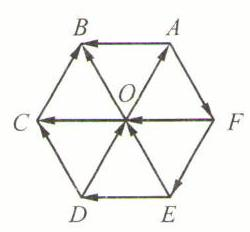
\includegraphics[width=0.2\textwidth]{bodyxb/src/bo_d20aucref24c73anc48g_5_1196_236_250_232_0.jpg}
\end{center}


(第 21 题)

22. 已知 $O$ 是平面上的一定点, $A,B,C$ 是平面上不共线的 3 个点,一动点 $P$ 满足: $\vv{OP} = \vv{OA} + \lambda \left( {\vv{AB} + \vv{AC}}\right) ,\lambda  > 0$ ,判断动点 $P$ 的轨迹是否经过 $\bigtriangleup {ABC}$ 的重心,并说明理由?

23. 已知点 $O$ 为 $\bigtriangleup {ABC}$ 内一点,且 $\angle {AOB} = \angle {BOC} = \angle {COA} = {120}^{ \circ  }$ . 求证: $\left| \vv{OA}\right|  = \left| \vv{OB}\right|  = \left| \vv{OC}\right|$ 的充要条件为: $\vv{OA} + \vv{OB} + \vv{OC} = \vv{0}$ .

\section*{二、向量的数量积}

\section*{【典型例题和解题技巧】}

\section*{1. 向量的投影.}

如果向量 $\vv{AB}$ 的起点 $A$ 和终点 $B$ 在直线 $l$ 上的投影分别为 ${A}^{\prime }$ 和 ${B}^{\prime }$ ,称向量 $\vv{{A}^{\prime }{B}^{\prime }}$ 叫做向量 $\vv{AB}$ 在直线 $l$ 上的投影向量,简称投影. 实数 $\left| \vv{b}\right| \cos \langle \vv{a},\vv{b}\rangle$ 称为向量 $\vv{b}$ 在向量 $\vv{a}$ 方向上的数量投影.

例 1 已知向量 $a,b$ 满足: $\left| \vv{a}\right|  = 2,\left| \vv{b}\right|  = \sqrt{3},\left| {\vv{a} + \vv{b}}\right|  = \sqrt{2}$ ,求向量 $\vv{a} - \vv{b}$ 在向量 $\vv{a} + \vv{b}$ 方向上的数量投影.

解 利用数量投影的定义,向量 $\vv{a} - \vv{b}$ 在向量 $\vv{a} + \vv{b}$ 方向上的数量投影为:

$\left| {\vv{a} - \vv{b}}\right| \cos \langle \vv{a} - \vv{b},\vv{a} + \vv{b}\rangle  = \dfrac{\left( {\vv{a} - \vv{b}}\right)  \cdot  \left( {\vv{a} + \vv{b}}\right) }{\left| \vv{a} + \vv{b}\right| } = \dfrac{{\left| \vv{a}\right| }^{2} - {\left| \vv{b}\right| }^{2}}{\sqrt{2}} = \dfrac{4 - 3}{\sqrt{2}} = \dfrac{\sqrt{2}}{2}$ .

2. 直接用定义求数量积.

若非零向量 $a,b$ 的夹角为 $\theta$ ,则 $\left| a\right| \left| b\right| \cos \theta$ 叫做向量 $a,b$ 的数量积.

记作 $\vv{a} \cdot  \vv{b} = \left| \vv{a}\right| \left| \vv{b}\right| \cos \theta$ ,其中 $\theta$ 是 $\vv{a}$ 与 $\vv{b}$ 的夹角. 数量积又称内积.

规定:零向量与任何一个向量的数量积为 0 .

例 2 已知 $\left| \vv{a}\right|  = 4,\left| \vv{b}\right|  = 5$ ,分别求下列条件下 $\vv{a}$ 与 $\vv{b}$ 的数量积:

(1) $\vv{a}//\vv{b}$ ； (2) $a\bot b$ ； (3) $a$ 与 $b$ 的夹角为 ${120}^{ \circ  }$ .

解 (1) 当 $a$ 与 $b$ 同向时, $\theta  = {0}^{ \circ  },a \cdot  b = \left| a\right| \left| b\right|  = {20}$ ;

当 $a$ 与 $b$ 反向时, $\theta  = {180}^{ \circ  },a \cdot  b =  - \left| a\right| \left| b\right|  =  - {20}$ .

(2)当 $\vv{a}\bot \vv{b}$ 时, $\theta  = {90}^{ \circ  }$ , $\vv{a} \cdot  \vv{b} = 0$ .

(3) $\vv{a} \cdot  \vv{b} = \left| \vv{a}\right|  \cdot  \left| \vv{b}\right| \cos {120}^{ \circ  } =  - {10}$ .

注意 当 $a//b$ 时,需分 $a$ 与 $b$ 同向和反向两种情况讨论.

3. 利用数量积求向量的模.

$\left| a\right|  = \sqrt{a \cdot  a}.$

例 3 已知 $\left| \vv{a}\right|  = 3\sqrt{3},\left| \vv{b}\right|  = 1$ ,且 $\vv{a}$ 与 $\vv{b}$ 的夹角为 ${150}^{ \circ  }$ ,试求 $\left| {\vv{a} - 2\vv{b}}\right|$ .

解 $\because {\left| a - 2b\right| }^{2} = {\left( a - 2b\right) }^{2} = {a}^{2} - {2a} \cdot  {2b} + {\left( 2b\right) }^{2} = {27} - 4 \times  3\sqrt{3} \times  1 \times  \cos {150}^{ \circ  } + 4 = {49}$ ,

$\therefore \left| {a - {2b}}\right|  = 7$ .

注意 求向量模的常用方法是平方法,即利用 ${\left| a\right| }^{2} = {a}^{2}$ 来求解.

4. 求与两个向量的夹角、垂直有关的问题.

(1)若向量 $a$ 与 $b$ 的夹角为 $\theta$ ,则有 $\cos \theta  = \dfrac{a \cdot  b}{\left| a\right| \left| b\right| }$ .

(2)若 $a$ 与 $b$ 是两个非零向量,则有 $a\bot b \Leftrightarrow  a \cdot  b = 0$ .

例 4 已知 $\left| \vv{a}\right|  = \sqrt{3},\left| \vv{b}\right|  = 2$ ,且 $\vv{a}$ 与 $\vv{b}$ 的夹角为 $\dfrac{\pi }{6}$ ,试求 $\vv{a} + 2\vv{b}$ 与 $\vv{a} - \vv{b}$ 的夹角的余弦值.

解 $a \cdot  b = \left| a\right| \left| b\right| \cos \dfrac{\pi }{6} = 3$ .

$\because {\left| \vv{a} + 2\vv{b}\right| }^{2} = {\left( \vv{a} + 2\vv{b}\right) }^{2} = {\vv{a}}^{2} + 4\left( {\vv{a} \cdot  \vv{b}}\right)  + 4{\vv{b}}^{2} = 3 + 4 \times  3 + 4 \times  4 = {31},$

$\therefore \left| {a + {2b}}\right|  = \sqrt{31}$ .

$\because {\left| a - b\right| }^{2} = {\left( a - b\right) }^{2} = {a}^{2} - 2\left( {a \cdot  b}\right)  + {b}^{2} = 3 - 2 \times  3 + 4 = 1,\therefore \left| {a - b}\right|  = 1$ .

$\because \left( {\vv{a} + 2\vv{b}}\right)  \cdot  \left( {\vv{a} - \vv{b}}\right)  = {\vv{a}}^{2} + \vv{a} \cdot  \vv{b} - 2{\vv{b}}^{2} = 3 + 3 - 2 \times  4 =  - 2$ ,

$\therefore \cos \theta  = \dfrac{-2}{\sqrt{31} \times  1} =  - \dfrac{2\sqrt{31}}{31}.\therefore \vv{a} + 2\vv{b}$ 与 $\vv{a} - \vv{b}$ 的夹角的余弦值为 $- \dfrac{2\sqrt{31}}{31}$ .

例 5 已知 $\left| \vv{a}\right|  = \sqrt{2},\left| \vv{b}\right|  = 3,\vv{a}$ 与 $\vv{b}$ 的夹角为 ${45}^{ \circ  }$ ,当向量 $\vv{a} + \vv{b}$ 与 $\lambda \vv{a} + \vv{b}$ 的夹角为锐角时, 求实数 $\lambda$ 的取值范围.

解 $\because a + b$ 与 ${\lambda a} + b$ 的夹角为锐角, $\therefore \left( {a + b}\right)  \cdot  \left( {{\lambda a} + b}\right)  > 0$ ,

即 $\lambda {\vv{a}}^{2} + \left( {1 + \lambda }\right) \vv{a} \cdot  \vv{b} + {\vv{b}}^{2} > 0$ .

$\because a \cdot  b = \sqrt{2} \times  3 \times  \cos {45}^{ \circ  } = 3,\therefore {5\lambda } + {12} > 0$ ,得 $\lambda  >  - \dfrac{12}{5}$ .

易知当 $\lambda  = 1$ 时, $\vv{a} + \vv{b}$ 与 $\lambda \vv{a} + \vv{b}$ 的夹角为 ${0}^{ \circ  }$ ,

$\therefore \lambda  \neq  1$ ,从而得 $\lambda  \in  \left( {-\dfrac{12}{5},1}\right)  \cup  \left( {1, + \infty }\right)$ . $\left\lbrack  {0,\dfrac{\pi }{2}}\right)$

注意 当两个向量的数量积大于 0 时, 它们的夹角取值范围是

例 6 已知 $a,b$ 是两个非零向量, $t$ 为实数,且 $\mu  = a + {tb}$ .

(1)当 $\left| \mathbf{\mu }\right|$ 取最小值时,求实数 $t$ 的值； (2)当 $\left| \mathbf{\mu }\right|$ 取最小值时,求证: $\vv{b} \bot  \left( {\vv{a} + t\vv{b}}\right)$ .

(1)解 ∵ ${\left| \mathbf{\mu }\right| }^{2} = {\left( \vv{a} + t\vv{b}\right) }^{2} = {\left| \vv{b}\right| }^{2}{t}^{2} + {2t}\left( {\vv{a} \cdot  \vv{b}}\right)  + {\left| \vv{a}\right| }^{2}$

$= {\left| \vv{b}\right| }^{2}{\left( t + \dfrac{\vv{a} \cdot  \vv{b}}{{\left| \vv{b}\right| }^{2}}\right) }^{2} + {\left| \vv{a}\right| }^{2} - {\left( \dfrac{\vv{a} \cdot  \vv{b}}{\left| \vv{b}\right| }\right) }^{2},$

$\therefore$ 当 $t =  - \dfrac{\vv{a} \cdot  \vv{b}}{{\left| \vv{b}\right| }^{2}}$ 时, $\left| \mathbf{\mu }\right|$ 最小.

(2)证明 $\because b \cdot  \left( {a + {tb}}\right)  = b \cdot  a + t{b}^{2} = b \cdot  a - \dfrac{a \cdot  b}{{\left| b\right| }^{2}}{\left| b\right| }^{2} = 0$ ,

$\therefore b \bot  \left( {a + {tb}}\right)$ .

5. 与其他知识的综合.

例 7 如图 2,已知 $\bigtriangleup {OAB}$ 的面积为 $S$ ,且 $\vv{OA} \cdot  \vv{AB} = 2$ .

(1)若 $1 < S < \sqrt{3}$ ,求向量 $\vv{OA}$ 与 $\vv{AB}$ 的夹角 $\theta$ 的取值范围；

(2)若 $\theta  \in  \left\lbrack  {\dfrac{\pi }{6},\dfrac{\pi }{3}}\right\rbrack$ ,求 $\bigtriangleup {OAB}$ 的最长边长的最小值.

解(1)由 $\vv{OA} \cdot  \vv{AB} = 2$ ,得 ${OA} \cdot  {AB} \cdot  \cos \theta  = 2$ .

\begin{center}
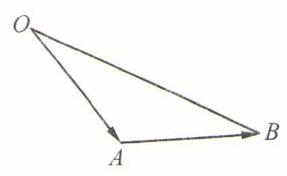
\includegraphics[width=0.2\textwidth]{bodyxb/src/bo_d20aucref24c73anc48g_7_1135_477_287_176_0.jpg}
\end{center}


(图 2)

由 $1 < S < \sqrt{3}$ ,得 $1 < \dfrac{1}{2} \cdot  {OA} \cdot  {AB} \cdot  \sin \theta  < \sqrt{3}$ .

$\therefore 1 < \dfrac{1}{2} \cdot  \dfrac{2}{\cos \theta } \cdot  \sin \theta  < \sqrt{3},\therefore 1 < \tan \theta  < \sqrt{3}$ .

$\because 0 < \theta  < \pi ,\therefore \dfrac{\pi }{4} < \theta  < \dfrac{\pi }{3}.$

(2)由已知,得 ${OB}$ 为 $\bigtriangleup {OAB}$ 的最长边.

$\because \vv{OB} = \vv{OA} + \vv{AB}$ ,

$\therefore {\left| \vv{OB}\right| }^{2} = {\vv{OB}}^{2} = {\left( \vv{OA} + \vv{AB}\right) }^{2} = {\vv{OA}}^{2} + {\vv{AB}}^{2} + 2\vv{OA} \cdot  \vv{AB} = {\left| \vv{OA}\right| }^{2} + {\left| \vv{AB}\right| }^{2} + 4$  $\geq  2\left| \vv{OA}\right|  \cdot  \left| \vv{AB}\right|  + 4 = \dfrac{4}{\cos \theta } + 4.$

$\because \theta  \in  \left\lbrack  {\dfrac{\pi }{6},\dfrac{\pi }{3}}\right\rbrack  ,\therefore \dfrac{1}{2} \leq  \cos \theta  \leq  \dfrac{\sqrt{3}}{2},\therefore {\left| \vv{OB}\right| }^{2} \geq  \dfrac{8\sqrt{3}}{3} + 4$ .

$\therefore \left| \vv{OB}\right|  \geq  \dfrac{2}{3}\sqrt{9 + 6\sqrt{3}}$ ,即 ${OB}$ 的最小值为 $\dfrac{2}{3}\sqrt{9 + 6\sqrt{3}}$ .

注意 在 $\bigtriangleup {OAB}$ 中,向量 $\vv{OA}$ 与 $\vv{AB}$ 的夹角不是角 $A$ ,而是其补角.

\section*{【训练题】}

\section*{(A)}

24. 若 $\left| \vv{a}\right|  = 1,\left| \vv{b}\right|  = 4,\vv{a}$ 与 $\vv{b}$ 的夹角为 ${30}^{ \circ  }$ ,则 $\vv{a} \cdot  \vv{b}$ 的值为 (C)

(A) $\dfrac{\sqrt{3}}{2}$ . (B) $\sqrt{3}$ . (C) $2\sqrt{3}$ . (D) $\dfrac{1}{2}$ .

25. 已知 $\vv{a},\vv{b}$ 均为单位向量,它们的夹角为 ${60}^{ \circ  }$ ,那么 $\left| {\vv{a} + 3\vv{b}}\right|$ 等于 (C) $\left( {\dfrac{1}{2},\dfrac{\sqrt{2}}{2}}\right)$

(A) $\sqrt{7}$ . (B) $\sqrt{10}$ . (C) $\sqrt{13}$ . (D) $4.\left( {\dfrac{3}{2},\dfrac{0}{2}}\right)$ 26. 设 $m,n$ 为非零向量,则 “存在负数 $\lambda$ ,使得 $m = {\lambda n}$ ” 是 “ $m \cdot  n < 0$ ” 的 ( $A$ )

(A) 充分而不必要条件 (B) 必要而不充分条件

(C) 充分必要条件 (D) 既不充分也不必要条件

27. 已知单位向量 $a,b$ 的夹角为 ${60}^{ \circ  }$ ,则在下列向量中,与 $b$ 垂直的是 (   )

(A) $a + {2b}$ . (B) ${2a} + b$ . (C) $a - {2b}$ . (D) ${2a} - b$ .

$\left| \vv{a}\right|  \cdot  \left| \vv{b}\right|  \cdot  \cos \theta  = {\left| \vv{b}\right| }^{2}$

$\vv{a} \cdot  \vv{b} = {\left| \vv{b}\right| }^{2}$

28. 已知非零向量 $\vv{a},\vv{b}$ 满足 $\left| \vv{a}\right|  = 2\left| \vv{b}\right|$ ,且 $\left( {\vv{a} - \vv{b}}\right) \bot \vv{b}$ ,则 $\vv{a}$ 与 $\vv{b}$ 的夹角为(B)

(A) $\dfrac{\pi }{6}$ . (B) $\dfrac{\pi }{3}$ . (C) $\dfrac{2\pi }{3}$ . (D) $\dfrac{5\pi }{6}$ .

29. 下列结论正确的是(A)

(A) ${\left| a\right| }^{2} = a \cdot  a$ . (B) $\left( {a \cdot  b}\right) \left( {a \cdot  b}\right)  = \left( {a \cdot  a}\right) \left( {b \cdot  b}\right)$ .

(C) 若 $a \cdot  b = 0$ ,则 $a = 0$ 或 $b = 0$ . (D) $\left| {a \cdot  b}\right|  = \left| a\right|  \cdot  \left| b\right|$ .

30. 若平面上 ${P}_{1},{P}_{2},{P}_{3}$ 三点满足 $\vv{O{P}_{1}} + \vv{O{P}_{2}} + \vv{O{P}_{3}} = \vv{0}$ ,且 $\left| \vv{O{P}_{1}}\right|  = \left| \vv{O{P}_{2}}\right|  = \left| \vv{O{P}_{3}}\right|$ ,则 $\bigtriangleup {P}_{1}{P}_{2}{P}_{3}$ 的形状是 (   )

(A) 钝角三角形. (B) 直角三角形. (C) 等腰三角形. (D) 等边三角形.

31. 若 $A,B,C,D$ 是平面上不共线的四点,则 “ $\vv{AB}$ 与 $\vv{CD}$ 共线”是 “ $\vv{AB} \cdot  \vv{BC} = \vv{BC} \cdot  \vv{CD} = 0$ ” 的(B)

(A) 充分不必要条件. (B) 必要不充分条件.

(C) 充要条件. (D) 既不充分也不必要条件.

若 $O$ 是 $\bigtriangleup {ABC}$ 所在平面上一点, $\vv{OA} \cdot  \vv{OB} = \vv{OB} \cdot  \vv{OC} = \vv{OC} \cdot  \vv{OA}$ ,则点 $O$ 是 $\bigtriangleup {ABC}$ 的(B)

(A) 重心. (B) 垂心. (C) 内心. (D) 外心.

33. 若向量 $a,b$ 的夹角为 ${60}^{ \circ  },\left| \vv{a}\right|  = 3,\left| \vv{b}\right|  = 2,\left( {{3a} + {5b}}\right)  \bot  \left( {{ma} - b}\right)$ ,则实数 $m$ 的值为 (   )

(A) $\dfrac{32}{23}$ . (B) $\dfrac{29}{42}$ . (C) $\dfrac{23}{42}$ .

34. 若 $a$ 与 $b - c$ 都是非零向量,则 “ $a \cdot  b = a \cdot  c$ ” 是 “ $a \bot  {\left( b - c\right) }^{1/b}$ 的(C) ${42m} = {29}$

(A) 充分不必要条件. (B) 必要不充分条件.

(C) 充要条件. (D) 既不充分也不必要条件.

在 $\bigtriangleup {ABC}$ 中, $\angle A = {90}^{ \circ  },{AB} = 1,{AC} = 2$ . 设点 $P,Q$ 满足 $\vv{AP} = \lambda \vv{AB},\vv{AQ} = \left( {1 - \lambda }\right) \vv{AC},\lambda  \in$ R. 若 $\vv{BQ} \cdot  \vv{CP} =  - 2$ ,则 $\lambda  = \left( \begin{matrix} 3 \\  2 \end{matrix}\right)$ (A) $\dfrac{1}{3}$ . (B) $\dfrac{2}{3}$ . $= \left( {\vv{BA} + \vv{AQ}}\right) .\left( {\vv{CA} + \vv{AP}}\right)$  $= A\left( {\left( {1 - \lambda }\right) \vv{AC} - \vv{AB}}\right)  \cdot  \left( {\lambda \vv{AB} - \vv{AC}}\right)$

(C) $\dfrac{4}{3}$ . ${\left| \vv{a}\right| }^{2} + {\left| \vv{b}\right| }^{2} - 2\vv{a} \cdot  \vv{b} = 6$ (D) 2. $=  - \lambda {\left| \vv{AB}\right| }^{2} - \left( {1 - \lambda }\right) {\left| \vv{AC}\right| }^{2}$  ${\left| \vv{a}\right| }^{2} + {\left| \vv{b}\right| }^{2} + 2\vv{a} \cdot  \vv{b} = {10}$  $- x - 4\left( {1 - x}\right)$ 江 设向量 $\vv{a},\vv{b}$ 满足 $\left| {\vv{a} + \vv{b}}\right|  = \sqrt{10},\left| {\vv{a} - \vv{b}}\right|  = \sqrt{6}$ ,则 $\vv{a} \cdot  \vv{b} = 1$  $= {3x} - 4 =  - 2$

$2{\left| \vv{a}\right| }^{2} + \vv{a} \cdot  \vv{b} - 2\vv{a} \cdot  \vv{b} - \left| \vv{b}\right|  =  - 4$  $4 - 8\cos \theta  - {16} =  - 48\cos \theta  =  - {14}$

38. 已知 $A,B,C$ 是圆 $O$ 上的三点,若 $\vv{AQ} = \dfrac{1}{2}\left( {\vv{AB} + \vv{AC}}\right)$ ,则 $\vv{AB}$ 与 $\vv{AC}$ 的夹角为\blkda{}

$\sqrt{3} = \dfrac{1}{2} \times  4 \times  6$ 平面 $\sin \theta \sin \theta  = \dfrac{\sqrt{3}}{2}\cos \theta  = \dfrac{1}{2}$

39. 在锐角三角形 ${ABC}$ 中, $\left| \vv{AB}\right|  = 4$ , $\left| \vv{AC}\right|  = 1$ , ${S}_{\bigtriangleup {ABC}} = \sqrt{3}$ ,则 $\vv{AB} \cdot  \vv{AC} =$ \blkda{}2\blkda{}.

40. 设四边形 ${ABCD}$ 为平行四边形,

$2\vv{NC}$ ,则 $\vv{AM} \cdot  \vv{NM} =$ \blkda{}图9. 4. $\dfrac{1}{6} - \dfrac{3}{13}m$  $\vv{AM} \cdot  \vv{NM} = \left( {\vv{AB} + \vv{BM}}\right)  \cdot  \left( {\vv{NC} + \vv{CM}}\right)$ 若 $a$ 与 $b$ 的夹角为 ${120}^{ \circ  }$ ,且 $\left| a\right|  = 2,\left| b\right|  = 5$ ,则 $\left( {{2a} - b}\right)  \cdot  a = {13}$ . 令 $b$  $= \dfrac{1}{3}{\left( \vv{AB}\right) }^{2} + \dfrac{3}{16}{\left( \vv{BC}\right) }^{2}$  $= {12} + 3$  $\left( {\vv{AB} + \lambda \vv{BC}}\right)  \cdot  \left( {\vv{AD} + \mu \vv{DC}}\right)$  $4 + \vv{CA} \cdot  \left( {\vv{AE} + \vv{AF}}\right)  + 1 =  - \dfrac{2}{3}$  $= \vv{AB} \cdot  \vv{AD} + \lambda \vv{BC} \cdot  \vv{AD} + \mu \vv{AB} \cdot  \vv{DC}$  $\vv{CA} \cdot  \left( {\vv{AE} + \vv{AF}}\right)  =  - \dfrac{17}{2}$  $+ {\pi \mu BC} \cdot  {OC}$  $= \dfrac{1}{2} + {4\lambda } + {4\mu } + {2\lambda \mu } = 1$ 4. 已知菱形 ${ABCD}$ 的边长为 $2,\angle {BAD} = {120}^{ \circ  }$ ,点 $E$ , $F$ 分别在边 ${BCDC}$ 上, ${BE} = {\lambda BC},{DF}$  $\vv{CE} \cdot  \vv{CF} = \left( {1 - \lambda }\right) \vv{CB} + \left( {1 - \mu }\right) \vv{CD} = \left( {1 - \lambda }\right)  \cdot  \left( {1 - \mu }\right)  \cdot  \left( {1 - 2}\right)  =  - \dfrac{2}{3} \cdot  \lambda  + \mu  = \lambda  - \mu  + \dfrac{2}{3}{4\lambda \mu } + {3}^{-1} \cdot  {5}^{-1}A\vv{AB} \cdot  \vv{AC}$  $= {\mu DC}$ . 若 $\vv{AE} \cdot  \vv{AF} = 1,\vv{CE} \cdot  \vv{CF} =  - \dfrac{2}{3}$ ,则 $\lambda  + \mu  = \dfrac{1}{12}\vv{6}$ . A. ${2\lambda } + {2\mu } + {\lambda \mu } = \dfrac{1}{4}\left( {1 - \lambda }\right) \left( {1 - \mu }\right)  = \dfrac{1}{3}{\lambda \mu } - \left( {\lambda  + \mu }\right)  =  - \dfrac{2}{3}\lambda  + {3\mu } = \dfrac{1}{4} + \dfrac{5}{3} = \dfrac{11}{12}B - \dfrac{1}{5}\lambda  = 1$

$= 8 + 5$

44. 在 $\bigtriangleup {ABC}$ 中,设 $M$ 为边 ${BC}$ 的中点,且 $\left| \overline{AM}\right|  = 3,\left| \vv{BC}\right|  = {10}$ ,则 $\overline{AB} \cdot  \overline{AC} =  - {lb}$ .

45. 直角三角形 ${ABC}$ 中, ${AB} = 3,{AC} = 4,{BC} = 5,M$ 是 $\bigtriangleup {ABC}$ 外接圆上任意一点,则 $\vv{AB}$ . $\vv{AM}$ 的最大值为\blkda{}.

46. 在 $\bigtriangleup {ABC}$ 中, $\angle A = {60}^{ \circ  },{AB} = 3,{AC} = 2$ . 若 $\vv{BD} = 2\vv{DC},\vv{AE} = \lambda \vv{AC} - \vv{AB}\left( {\lambda  \in  \mathbf{R}}\right)$ ,且 $\vv{AD}$ . $\vv{AE} =  - 4$ ,则 $\lambda$ 的值为\blkda{}.

47. 在 $\bigtriangleup {ABC}$ 中, $\vv{CB} = \vv{a},\vv{CA} = \vv{b},\vv{a} \cdot  \vv{b} < 0,{S}_{\bigtriangleup {ABC}} = \dfrac{15}{4},\left| \vv{a}\right|  = 3,\left| \vv{b}\right|  = 5$ ,则 $\vv{a}$ 与 $\vv{b}$ 的夹角为\blkda{}.

48. 设 $a,b,c$ 是任意的非零向量,且它们两两不共线. 给出下列命题: ① $\left( {a \cdot  b}\right)  \cdot  c - \left( {c \cdot  a}\right)  \cdot  b$  $= 0$ ；② $\left| a\right|  - \left| b\right|  < \left| {a - b}\right|$ ；③ $\left( {b \cdot  c}\right)  \cdot  a - \left( {c \cdot  a}\right)  \cdot  b$ 不与 $c$ 垂直；④ $\left( {{3a} + {2b}}\right)  \cdot  \left( {{3a} - {2b}}\right)$  $= 9{\left| \vv{a}\right| }^{2} - 4{\left| \vv{b}\right| }^{2}$ . 其中真命题是\blkda{}(填序号).

49. 若 $a$ 与 $b$ 不平行,且 $a \cdot  b \neq  0$ ,记 $c = a - \left( \dfrac{a \cdot  a}{a \cdot  b}\right) b$ ,则向量 $a$ 与 $c$ 的夹角为\blkda{}.

50. 已知 $\left| \vv{a}\right|  = 4,\left| \vv{b}\right|  = {10},\vv{a}$ 与 $\vv{b}$ 的夹角为 ${60}^{ \circ  }$ ,求 $\left| {2\vv{a} - \vv{b}}\right|$ .

51. 已知向量 $\vv{a}$ 与 $\vv{b}$ 满足 $\left| \vv{a}\right|  = \left| \vv{b}\right|  = 1,\left| {3\vv{a} - 2\vv{b}}\right|  = \sqrt{7}$ .

(1)求 $a$ 与 $b$ 的夹角； (2)求 $\left| {{3a} + b}\right|$ .

52. 已知向量 $a,b,x,y$ 满足 $a = y - x,b = {2x} - y,\left| a\right|  = \left| b\right|  = 1$ ,且 $a \bot  b$ .

(1)用 $a,b$ 表示 $x,y$ ； (2) 求 $\left| \mathbf{x}\right|$ 和 $\left| \mathbf{y}\right|$ .

53. 在 $\bigtriangleup {OAB}$ 中, $\vv{OA} = \vv{a},\vv{OB} = \vv{b},{OD}$ 是 ${AB}$ 边上的高,若 $\vv{AD} = \lambda \vv{AB}$ ,求实数 $\lambda$ 的值 (用 $\vv{a},b$ 表示).

54. 在 $\bigtriangleup {OAB}$ 中,非零向量 $\vv{OA} = \vv{a},\vv{OB} = \vv{b}$ ,若点 $B$ 关于 $\vv{OA}$ 所在直线的对称点为 ${B}_{1}$ ,求向量 $\vv{O{B}_{1}}$ (用 $\vv{a},\vv{b}$ 表示).

\begin{center}
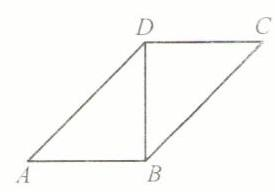
\includegraphics[width=0.2\textwidth]{bodyxb/src/bo_d20aucref24c73anc48g_9_1161_1399_275_192_0.jpg}
\end{center}


(第 55 题)

55. 如图,在四边形 ${ABCD}$ 中, $\left| \vv{AB}\right|  + \left| \vv{BD}\right|  + \left| \vv{DC}\right|  = 4,\vv{AB} \cdot  \vv{BD} =$  $\vv{BD} \cdot  \vv{DC} = 0,\left| \vv{AB}\right|  \cdot  \left| \vv{BD}\right|  + \left| \vv{BD}\right|  \cdot  \left| \vv{DC}\right|  = 4$ ,求 $\left( {\vv{AB} + \vv{DC}}\right)$ . $\vv{AC}$ 的值.

\section*{(B)}

56. 设平面上有四个互异的点 $A,B,C,D$ ,且 $\left( {\vv{DB} + \vv{DC} - 2\vv{DA}}\right)  \cdot  \left( {\vv{AB} - \vv{AC}}\right)  = 0$ ,则 $\bigtriangleup  {ABC}$ 的形状是(   )

(A) 直角三角形. (B) 等腰三角形. (C) 等腰直角三角形. (D) 等边三角形.

57. $\bigtriangleup {ABC}$ 是边长为 2 的等边三角形,已知向量 $a,b$ 满足 $\vv{AB} = {2a},\vv{AC} = {2a} + b$ ,则下列结论正确的是(   )

(A) $\left| \vv{b}\right|  = 1$ . (B) $a\bot b$ . (C) $a \cdot  b = 1$ . (D) $\left( {4\vv{a} + \vv{b}}\right)  \bot  \vv{BC}$ .

58. 已知 $\bigtriangleup {ABC}$ 是边长为 2 的等边三角形, $P$ 为平面 ${ABC}$ 内一点,则 $\vv{PA} \cdot  \left( {\vv{PB} + \vv{PC}}\right)$ 的最小值是(   )

(A) -2 . (B) $- \dfrac{3}{2}$ . (C) $- \dfrac{4}{3}$ . (D) -1 .

59. 若 $\left| \mathbf{p}\right|  = 2\sqrt{2},\left| \mathbf{q}\right|  = 3,\mathbf{p}$ 与 $\mathbf{q}$ 的夹角为 $\dfrac{\pi }{4}$ ,则以 $\vv{a} = \mathbf{{5p}} + 2\mathbf{q},\vv{b} = \mathbf{p} - 3\mathbf{q}$ 为邻边的平行四边形的一条对角线的长为 (   )

(A) 15. (B) $\sqrt{15}$ . (C) 14. (D) 16.

60. 若 $\left| \vv{a}\right|  = \left| \vv{b}\right|  = 1,\vv{a} \bot  \vv{b},\left( {{2\vv{a}} + {3\vv{b}}}\right)  \bot  \left( {{ka} - {4\vv{b}}}\right)$ ,则实数 $k$ 的值为 (   )

(A) -6. (B) 6. (C)-3. (D) 3.

61. 若 $i,j$ 为互相垂直的单位向量, $a = i - {2j},b = i + {\lambda j}$ ,且 $a$ 与 $b$ 的夹角为锐角,则实数 $\lambda$ 的取值范围是(   )

(A) $\left( {\dfrac{1}{2}, + \infty }\right)$ . (B) $\left( {-\infty , - 2}\right)  \cup  \left( {-2,\dfrac{1}{2}}\right)$ .

(C) $\left( {-2,\dfrac{2}{3}}\right)  \cup  \left( {\dfrac{2}{3}, + \infty }\right)$ . (D) $\left( {-\infty ,\dfrac{1}{2}}\right)$ .

62. 如图,向量 $\vv{OA} = \vv{a},\vv{OC} = \vv{b}$ ,且 $\vv{CD}\bot \vv{OA},D$ 为垂足. 若 $\vv{OD} = \lambda \vv{a}$ ( $\lambda$  $\neq  0)$ ,则实数 $\lambda$ 的值为 (   )

\begin{center}
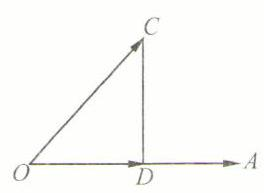
\includegraphics[width=0.2\textwidth]{bodyxb/src/bo_d20aucref24c73anc48g_10_1217_998_264_193_0.jpg}
\end{center}


(第 62 题)

(A) $\dfrac{\vv{a} \cdot  \vv{b}}{{\left| \vv{a}\right| }^{2}}$ . (B) $\dfrac{a \cdot  b}{\left| a\right|  \cdot  \left| b\right| }$ .

(C) $\dfrac{\vv{a} \cdot  \vv{b}}{{\left| \vv{b}\right| }^{2}}$ . (D) $\dfrac{a \cdot  b}{a \cdot  b}$ .

63. 若 $\left| \vv{a}\right|  = 3,\left| \vv{b}\right|  = 4$ ,则向量 $\vv{a} + \dfrac{3}{4}\vv{b}$ 与 $\vv{a} - \dfrac{3}{4}\vv{b}$ 的位置关系是 (   )

(A) 平行. (B) 垂直. (C) 夹角为 $\dfrac{\pi }{3}$ . (D) 不平行也不垂直.

64. 设 $\vv{a},\vv{b}$ 为非零向量, $\left| \vv{b}\right|  = 2\left| \vv{a}\right|$ ,两组向量 ${\mathbf{x}}_{1},{\mathbf{x}}_{2},{\mathbf{x}}_{3},{\mathbf{x}}_{4}$ 和 ${\mathbf{y}}_{1},{\mathbf{y}}_{2},{\mathbf{y}}_{3},{\mathbf{y}}_{4}$ 均由 2 个 $\vv{a}$ 和 2 个 $b$ 排列而成,若 ${x}_{1} \cdot  {y}_{1} + {x}_{2} \cdot  {y}_{2} + {x}_{3} \cdot  {y}_{3} + {x}_{4} \cdot  {y}_{4}$ 所有可能取值中的最小值为 $4{\left| a\right| }^{2}$ , 则 $a$ 与 $b$ 的夹角为(   )

(A) $\dfrac{2}{3}\pi$ . (B) $\dfrac{\pi }{3}$ . (C) $\dfrac{\pi }{6}$ . (D) 0 .

65. 设 $\theta$ 为两个非零向量 $a,b$ 的夹角,已知对任意实数 $t,\left| {b + {ta}}\right|$ 的最小值为 1 ,下列说法正确的是(   )

(A) 若 $\theta$ 确定,则 $\left| \vv{a}\right|$ 唯一确定. (B) 若 $\theta$ 确定,则 $\left| \vv{b}\right|$ 唯一确定.

(C) 若 $\left| \vv{a}\right|$ 确定,则 $\theta$ 唯一确定. (D) 若 $\left| \vv{b}\right|$ 确定,则 $\theta$ 唯一确定.

66. 若向量 $\vv{a} \neq  \vv{e}$ , $\left| \vv{e}\right|  = 1$ ,对任意的实数 $t$ ,都有 $\left| {\vv{a} - t\vv{e}}\right|  \geq  \left| {\vv{a} - \vv{e}}\right|$ 成立,则有(   )

(A) $a\bot e$ . (B) $\left( {a - e}\right) \bot a$ .

(C) $\left( {a - c}\right) \bot c$ . (D) $\left( {a + c}\right)  \bot  \left( {a - c}\right)$ .

67. 已知非零向量 $\vv{AB},\vv{AC}$ 满足 $\left( {\dfrac{\vv{AB}}{\left| \vv{AB}\right| } + \dfrac{\vv{AC}}{\left| \vv{AC}\right| }}\right)  \cdot  \vv{BC} = 0$ ,且 $\dfrac{\vv{AB}}{\left| \vv{AB}\right| } \cdot  \dfrac{\vv{AC}}{\left| \vv{AC}\right| } = \dfrac{1}{2}$ ,则 $\bigtriangleup  {ABC}$ 的形状是(   )

(A) 三边均不相等的三角形. (B) 直角三角形.

(C) 等腰三角形. (D) 等边三角形.

68. 在边长为 1 的等边三角形 ${ABC}$ 中,若 $\vv{BC} = \vv{a},\vv{CA} = \vv{b},\vv{AB} = \vv{c}$ ,则 $\vv{a} \cdot  \vv{b} + \vv{b} \cdot  \vv{c} + \vv{c} \cdot  \vv{a}$  $=$ \blkda{}.

69. 给出下列结论:①若 $a \neq  0,a \cdot  b = 0$ ,则 $b = 0$ ；②若 $a \cdot  b = b \cdot  c$ ,则 $a = c$ . 其中结论正确的个数是\blkda{}.

70. 已知 $\vv{a},\vv{b}$ 为两个非零向量. 给出下列条件:① ${\vv{a}}^{2} = {\vv{b}}^{2}$ ；② $\vv{a} \cdot  \vv{b} = {\vv{b}}^{2}$ ；③ $\left| \vv{a}\right|  = \left| \vv{b}\right|$ ,且 $\vv{a}//\vv{b}$ . 其中可以作为 $\vv{a} = \vv{b}$ 的必要不充分条件的是\blkda{}(填序号).

71. 关于平面向量 $a,b,c$ ,有下列三个命题: ① 若 $a = \left( {1,k}\right) ,b = \left( {-2,6}\right) ,a//b$ ,则 $k =  - 3$ ; ② 若非零向量 $a,b$ 满足 $\left| a\right|  = \left| b\right|  = \left| {a - b}\right|$ ,则 $a$ 与 $a + b$ 的夹角为 ${60}^{ \circ  }$ . 其中真命题是\blkda{} (填序号).

72. 平行四边形 ${ABCD}$ 的两条对角线相交于点 $M,P$ 是 ${MD}$ 的中点. 若 $\left| \vv{AB}\right|  = 2,\left| \vv{AD}\right|  = 1$ 且 $\angle {BAD} = {60}^{ \circ  }$ ,则 $\vv{AP} \cdot  \vv{CP} =$ \blkda{}.

73. 设 ${e}_{1},{e}_{2}$ 为单位向量,满足 $\left| {2{e}_{1} - {e}_{2}}\right|  \leq  \sqrt{2},a = {e}_{1} + {e}_{2},b = 3{e}_{1} + {e}_{2}$ ,设 $a,b$ 的夹角为 $\theta$ ,则 ${\cos }^{2}\theta$ 的最小值为\blkda{}.

74. 已知平面向量 $a,b,c$ 满足: $\left| a\right|  = \left| b\right|  = 2,\langle a,b\rangle  = \dfrac{\pi }{3},{c}^{2} - {2a} \cdot  c - b \cdot  c + 4 = 0$ ,那么 $\left( {\vv{a} + \vv{c}}\right)  \cdot  \vv{b}$ 的最大值为\blkda{}.

75. 在 $\bigtriangleup {ABC}$ 中, $\vv{AB} = \vv{c},\vv{BC} = \vv{a},\vv{CA} = \vv{b}$ ,又 $\left( {\vv{c} \cdot  \vv{b}}\right)  : \left( {\vv{b} \cdot  \vv{a}}\right)  : \left( {\vv{a} \cdot  \vv{c}}\right)  = 1 : 2 : 3$ ,则 $\bigtriangleup {ABC}$ 的三边长之比 $\left| \vv{a}\right|  : \left| \vv{b}\right|  : \left| \vv{c}\right|  =$ \blkda{}.

\begin{center}
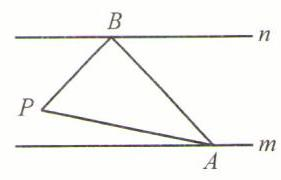
\includegraphics[width=0.2\textwidth]{bodyxb/src/bo_d20aucref24c73anc48g_11_1147_1376_281_180_0.jpg}
\end{center}


(第 76 题)

76. 如图,平面内点 $P$ 在两条平行直线 $m,n$ 之间,且到 $m,n$ 的距离分别为 1,2,点 $A,B$ 分别在直线 $m,n$ 上,且 $\left| {\vv{PA} + \vv{PB}}\right|  = 5$ ,则 $\vv{PA} \cdot  \vv{PB}$ 的最大值为\blkda{}.

77. 如图,在 $\bigtriangleup  {ABC}$ 中, $D$ 是 ${BC}$ 的中点, $E$ 在边 ${AB}$ 上, ${BE} = {2EA},{AD}$ 与 ${CE}$ 交于点 $O$ . 若 $\vv{AB} \cdot  \vv{AC} = 6\vv{AO} \cdot  \vv{EC}$ ,则 $\dfrac{AB}{AC}$ 的值是\blkda{}.

\begin{center}
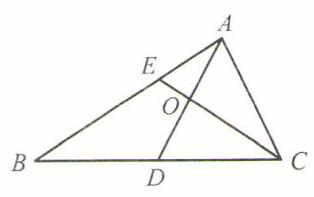
\includegraphics[width=0.2\textwidth]{bodyxb/src/bo_d20aucref24c73anc48g_11_1116_1658_314_197_0.jpg}
\end{center}


(第 77 题)

78. 已知 $a,b$ 是两个非零向量,且 $a + {3b}$ 与 ${7a} - {5b}$ 垂直, $a - {4b}$ 与 $7\vv{a} - 2\vv{b}$ 垂直,求 $\vv{a}$ 与 $\vv{b}$ 的夹角.

79. 已知 $\bigtriangleup {ABC}$ 的面积为 3,且 $0 \leq  \vv{AB} \cdot  \vv{AC} \leq  6$ . 设向量 $\vv{AB}$ 与 $\vv{AC}$ 的夹角为 $\theta$ . 求

(1) $\theta$ 的取值范围;

( 2 )函数 $f\left( \theta \right)  = 2{\sin }^{2}\left( {\dfrac{\pi }{4} + \theta }\right)  - \sqrt{3}\cos {2\theta }$ 的最大值和最小值.

80. 如图,在 $\mathrm{{Rt}} \bigtriangleup  {ABC}$ 中,已知 ${BC} = a$ . 若长为 ${2a}$ 的线段 ${PQ}$ 以点 $A$ 为中点,则 $\vv{PQ}$ 与 $\vv{BC}$ 的夹角 $\theta$ 取何值时, $\vv{BP} \cdot  \vv{CQ}$ 的值最大? 试求出这个最大值.

\begin{center}
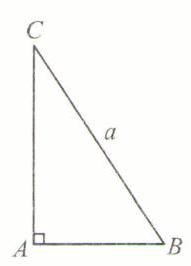
\includegraphics[width=0.2\textwidth]{bodyxb/src/bo_d20aucref24c73anc48g_12_1265_128_191_266_0.jpg}
\end{center}


(第 80 题)

81. 已知 $\bigtriangleup {ABC}$ 的三边长为 ${AB} = 5,{BC} = 6,{CA} = 7,G,I,O$ 分别为 $\bigtriangleup {ABC}$ 的重心、内心、外心,求 $\vv{AG} \cdot  \vv{BC},\vv{AI} \cdot  \vv{BC},\vv{AO} \cdot  \vv{BC}$ .

82. $A,B,C$ 为 $\bigtriangleup {ABC}$ 的内角, $G$ 为 $\bigtriangleup {ABC}$ 的重心,且 $\vv{GA} \cdot  \vv{GB} = 0$ ,求 $\cos C$ 的最小值.

83. 设 $\bigtriangleup {ABC},{P}_{0}$ 是边 ${AB}$ 上一定点,满足 $\vv{{P}_{0}B} = \dfrac{1}{4}\vv{AB}$ ,且对于边 ${AB}$ 上任一点 $P$ ,恒有 $\vv{PB} \cdot  \vv{PC} \geq  \vv{{P}_{0}B} \cdot  \vv{{P}_{0}C}$ . 求证: $\bigtriangleup {ABC}$ 是等腰三角形.

84. 已知向量 $a,b$ 满足: $\left| a\right|  = 1,\left| b\right|  = 2$ ,若对任意单位向量 $e$ ,均有 $\left| {a \cdot  e}\right|  + \left| {b \cdot  e}\right|  \leq  \sqrt{6}$ ,求 $\vv{a} \cdot  \vv{b}$ 的最大值.

85. 设 $S$ 是一些向量的集合,对于 $a \in  S$ ,如果 $a$ 的模长不小于 $S$ 中其余所有向量之和的长度, 则称 $a$ 是 $S$ 中的一个长向量. 对于 $S = \left\{  {{a}_{1},{a}_{2},\cdots ,{a}_{n}}\right\}  \left( {n > 2}\right)$ ,已知 $S$ 中每一个向量都是长向量,求证: ${a}_{1} + {a}_{2} + \cdots  + {a}_{n} = 0$ .

86. 平面上给定五个点 ${A}_{1},{A}_{2},{A}_{3},{A}_{4},{A}_{5}$ ,若点 $A$ 满足 $\vv{{A}_{1}{A}_{2}},\vv{{A}_{2}{A}_{3}},\vv{{A}_{3}{A}_{4}},\vv{{A}_{4}{A}_{5}},\vv{{A}_{5}A}$ 这五个向量中任意两个向量之和的模长等于其余三个向量之和的模长,证明: 点 $A$ 与点 ${A}_{1}$ 重合.

\section*{三、平面向量基本定理}

\section*{【典型例题和解题技巧】}

\section*{1. 平面向量的基本定理.}

平面向量的基本定理: 如果 ${e}_{1},{e}_{2}$ 是同一平面上的两个不共线向量,那么对于这一平面上的任意向量 $\vv{a}$ ,有且只有一对实数 ${\lambda }_{1},{\lambda }_{2}$ ,使 $\vv{a} = {\lambda }_{1}{\vv{e}}_{1} + {\lambda }_{2}{\vv{e}}_{2}$ .

例 1 如图 3,四边形 ${OADB}$ 是平行四边形,且 ${BM} = \dfrac{1}{3}{BC},{CN} = \dfrac{1}{3}$  ${CD}$ ,设 $\vv{OA} = \vv{a},\vv{OB} = \vv{b}$ 试用 $\vv{a},\vv{b}$ 表示 $\vv{OM},\vv{ON},\vv{MN}$ .

\begin{center}
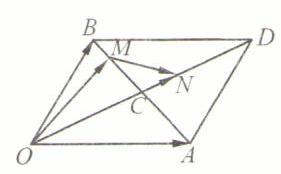
\includegraphics[width=0.2\textwidth]{bodyxb/src/bo_d20aucref24c73anc48g_12_1200_1601_281_174_0.jpg}
\end{center}


(图 3)

解 $\vv{OM} = \vv{OB} + \vv{BM} = \vv{OB} + \dfrac{1}{6}\vv{BA} = \vv{OB} + \dfrac{1}{6}\left( {\vv{OA} - \vv{OB}}\right)  =$

$\dfrac{1}{6}\vv{a} + \dfrac{5}{6}\vv{b},\vv{ON} = \dfrac{2}{3}\vv{OD} = \dfrac{2}{3}\left( {\vv{OA} + \vv{OB}}\right)  = \dfrac{2}{3}\vv{a} + \dfrac{2}{3}\vv{b},$

$\vv{MN} = \vv{ON} - \vv{OM} = \dfrac{1}{2}\vv{a} - \dfrac{1}{6}\vv{b}.$

注意 本例以不共线的两个向量 $\vv{OA} = \vv{a},\vv{OB} = \vv{b}$ 为基底来表示同一个平面上的其他向量.

2. 平面向量基本定理与三点共线的问题.

$A,B,C$ 三点共线 $\Leftrightarrow$ 存在唯一的实数 $\lambda$ ,使 $\vv{AB} = \lambda \vv{BC}$ .

例 2 设 ${\vv{e}}_{1},{\vv{e}}_{2}$ 是两个不共线的向量. 已知 $\vv{AB} = 2{\vv{e}}_{1} + k{\vv{e}}_{2},\vv{CB} = {\vv{e}}_{1} + 3{\vv{e}}_{2},\vv{CD} = 2{\vv{e}}_{1} - {\vv{e}}_{2}$ , 且 $A,B,D$ 三点共线,求实数 $k$ 的值.

解 $\because A,B,D$ 三点共线, $\therefore$ 存在实数 $\lambda$ ,使 $\vv{AB} = \lambda \vv{BD}$ .

$\because \vv{BD} = \vv{CD} - \vv{CB} = {\vv{e}}_{1} - 4{\vv{e}}_{2},\therefore 2{\vv{e}}_{1} + k{\vv{e}}_{2} = \lambda \left( {{\vv{e}}_{1} - 4{\vv{e}}_{2}}\right) .$

$\because {e}_{1},{e}_{2}$ 不共线, $\therefore \left\{  {\begin{array}{l} 2 = \lambda , \\  k =  - {4\lambda }. \end{array}\therefore k =  - 8}\right.$ .

例 3 如图 4,在 $\bigtriangleup {OAB}$ 中,点 $B$ 关于点 $A$ 的对称点是点 $C$ ,点 $D$ 是将线段 ${OB}$ 分成 $2 : 1$ 的两部分的一个内分点, ${DC}$ 与 ${OA}$ 交于点 $E$ ,设 $\vv{OA} = \vv{a},\vv{OB} = \vv{b}$ .

(1)用 $a$ 和 $b$ 表示向量 $\vv{OC},\vv{DC}$ ；

\begin{center}
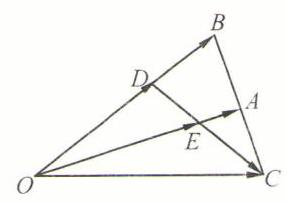
\includegraphics[width=0.2\textwidth]{bodyxb/src/bo_d20aucref24c73anc48g_13_1118_702_287_202_0.jpg}
\end{center}


(图 4)

(2)若 $\vv{OE} = \lambda \vv{OA}$ ,求实数 $\lambda$ 的值.

解 (1) $\vv{OC} = \vv{OA} + \vv{AC} = \vv{OA} + \vv{BA} = \vv{OA} + \vv{OA} - \vv{OB} = {2a} - b$ ,

$\vv{DC} = \vv{OC} - \vv{OD} = 2\vv{a} - \vv{b} - \dfrac{2}{3}\vv{b} = 2\vv{a} - \dfrac{5}{3}\vv{b}.$

(2) $\vv{EC} = \vv{OC} - \vv{OE} = 2\vv{a} - \vv{b} - \lambda \vv{a} = \left( {2 - \lambda }\right) \vv{a} - \vv{b}$ .

$\because \vv{EC}//\vv{DC},\therefore $ 存在实数 $\mu$ ,使 $\vv{EC} = \mu \vv{DC}$ .

$\therefore \left( {2 - \lambda }\right) \vv{a} - \vv{b} = \mu \left( {2\vv{a} - \dfrac{5}{3}\vv{b}}\right) ,\therefore \left\{  {\begin{array}{l} 2 - \lambda  = {2\mu }, \\   - 1 =  - \dfrac{5}{3}\mu . \end{array}\therefore \lambda  = \dfrac{4}{5}}\right.$ .

3. 利用平面向量基本定理证明平面几何问题.

例 4 用向量方法证明:平行四边形的一个顶点和对边中点的连线三等分此平行四边形的一条对角线.

证明 如图 5,设 $F$ 是 $▱{ABCD}$ 的边 ${CD}$ 的中点, $E$ 是 ${AF}$ 与 ${BD}$ 的交点.

$\because A,E,F$ 及 $B,E,D$ 均三点共线,

\begin{center}
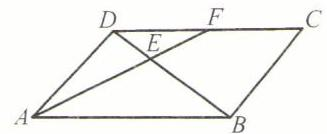
\includegraphics[width=0.2\textwidth]{bodyxb/src/bo_d20aucref24c73anc48g_13_1078_1445_327_134_0.jpg}
\end{center}


(图 5)

$\therefore$ 存在实数 $\lambda ,\mu$ ,使 $\vv{AE} = \lambda \vv{AF},\vv{BE} = \mu \vv{BD}$ .

$\because \vv{AE} = \vv{AB} + \vv{BE} = \vv{AB} + \mu \vv{BD} = \vv{AB} + \mu \left( {\vv{AD} - \vv{AB}}\right)$

$= \left( {1 - \mu }\right) \vv{AB} + \mu \vv{AD},\lambda \vv{AF} = \lambda \left( {\vv{AD} + \vv{DF}}\right)  = \lambda \left( {\vv{AD} + \dfrac{1}{2}\vv{AB}}\right)  = \dfrac{\lambda }{2}\vv{AB} + \lambda \vv{AD}$ ,

$\therefore \left( {1 - \mu }\right) \vv{AB} + \mu \vv{AD} = \dfrac{\lambda }{2}\vv{AB} + \lambda \vv{AD}$ .

$\because \vv{AB},\vv{AD}$ 不共线, $\therefore \left\{  {\begin{array}{l} 1 - \mu  = \dfrac{\lambda }{2}, \\  \mu  = \lambda  \end{array} \Rightarrow  \mu  = \dfrac{2}{3} \Rightarrow  \vv{BE} = \dfrac{2}{3}\vv{BD}}\right.$ ,

即 $E$ 是 ${BD}$ 的一个三等分点.

注意 选择 $\vv{AB},\vv{AD}$ 为基底,利用 $A,E,F$ 和 $B,E,D$ 两组三点共线,建立向量方程. 由平面向量基本定理,得到关于实数 $\lambda ,\mu$ 的方程组,解此方程组即可.

\section*{(A)}

87. 在 $\bigtriangleup {ABO}$ 中,设 $\vv{OA} = \vv{a},\vv{OB} = \vv{b}$ ,又 $\vv{OP} = m\vv{a} + n\vv{b}$ ,则下列命题正确的是 (   )

(A) 若 $m = n$ ,则点 $P$ 在 $\angle {AOB}$ 的平分线所在的直线上.

(B) 若 $m =  - n$ ,则点 $P$ 在边 ${AB}$ 所在的直线上.

(C) 若 $m = 0$ ,则点 $P$ 在边 ${OB}$ 所在的直线上.

(D) 若 $m \neq  0$ ,则点 $P$ 在边 ${OA}$ 所在的直线上.

88. 在 $\bigtriangleup {ABC}$ 中,点 $D$ 在边 ${BC}$ 上,且 $\vv{CD} = 2\vv{DB},\vv{CD} = r\vv{AB} + s\vv{AC}$ ,则 $r + s$ 的值为 (   )

(A) $\dfrac{2}{3}$ . (B) $\dfrac{4}{3}$ . (C)-3. (D) 0 .

89. 在 $\bigtriangleup {OAB}$ 中,设 $\vv{OA} = \vv{a},\vv{OB} = \vv{b},\vv{OP} = \mathbf{p}$ . 若 $\mathbf{p} = t\left( {\dfrac{a}{\left| \vv{a}\right| } + \dfrac{\vv{b}}{\left| \vv{b}\right| }}\right) ,t \in  \mathbf{R}$ ,则点 $P$ 在 (   )

(A) $\angle {AOB}$ 的平分线所在的直线上. (B) 线段 ${AB}$ 的垂直平分线上.

(C) 边 ${AB}$ 所在的直线上. (D) 边 ${AB}$ 的中线上.

90. 在平面直角坐标系中, $O$ 是坐标原点,两定点 $A,B$ 满足 $\left| \vv{OA}\right|  = \left| \vv{OB}\right|  = \vv{OA} \cdot  \vv{OB} = 2$ ,则点集 $\{ P\left| {\vv{OP} = \lambda \vv{OA} + \mu \vv{OB},}\right| \lambda \left| +\right| \mu  \mid   \leq  1,\lambda ,\mu  \in  \mathbf{R}\}$ 所表示的区域面积是 (   )

(A) $2\sqrt{2}$ . (B) $2\sqrt{3}$ . (C) $4\sqrt{2}$ . (D) $4\sqrt{3}$ .

91. 若向量 ${\vv{e}}_{1},{\vv{e}}_{2}$ 不共线, $2{\vv{e}}_{1} + 3{\vv{e}}_{2}$ 与 $k{\vv{e}}_{1} - 2{\vv{e}}_{2}$ 共线,则实数 $k$ 的值为\blkda{}.

92. 设 ${e}_{1},{e}_{2}$ 是两个不共线的向量,给出下列四组向量: ① ${e}_{1}$ 与 ${e}_{1} + {e}_{2}$ ; ② $3{e}_{1} - {e}_{2}$ 与 ${e}_{1} + {e}_{2}$ ; ③ ${e}_{1} - 2{e}_{2}$ 与 $6{e}_{2} - 3{e}_{1};$ ④ ${e}_{1} - 3{e}_{2}$ 与 ${e}_{1} + {e}_{2}$ . 可以作为平面内所有向量的一组基底的是\blkda{}. (填序号).

93. 若 $D,E$ 分别是 $\bigtriangleup {ABC}$ 的边 ${BC},{CA}$ 上的点,且 $\vv{BD} = \dfrac{1}{3}\vv{BC},\vv{CE} = \dfrac{1}{3}\vv{CA},\vv{AB} = a,\vv{AC} = b$ , 则 $\vv{DE} =$ \blkda{}.

94. 若向量 $\vv{a},\vv{b}$ 不共线, $m = \vv{a} + 2\vv{b},\vv{n} = 2\vv{a} + \lambda \vv{b}$ ,要使向量 $\vv{m},\vv{n}$ 能成为平面上所有向量的一组基底,则实数 $\lambda$ 的取值范围是\blkda{}.

95. 给出下列四个命题:①对于实数 $p$ 和向量 $a,b$ ,恒有 $p\left( {a - b}\right)  = {pa} - {pb}$ ；②对于实数 $p,q$ 和向量 $a$ ,恒有 $\left( {p - q}\right) a = {pa} - {qa}$ ；③对于实数 $p$ 和向量 $a,b$ ,若 ${pa} = {pb}$ ,则 $a = b$ ；④对于实数 $p,q$ 和向量 $a,a \neq  0$ ,若 ${pa} = {qa}$ ,则 $p = q$ . 其中真命题是\blkda{}(填序号).

96. 给定向量 $\vv{OA} = \vv{a},\vv{OB} = \vv{b}$ ,则 $\angle {AOB}$ 的平分线上的单位向量 $c =$ \blkda{}.(用 $\vv{a},\vv{b}$ 表示)

97. 如图,在同一个平面内,向量 $\vv{OA},\vv{OB},\vv{OC}$ 的模分别为 $1,1,\sqrt{2},\vv{OA}$ 与 $\vv{OC}$ 的夹角为 $\alpha$ ,且 $\tan \alpha  = 7,\vv{OB}$ 与 $\vv{OC}$ 的夹角为 ${45}^{ \circ  }$ . 若 $\vv{OC} = m\vv{OA} + n\vv{OB}$  $\left( {m,n \in  \mathbf{R}}\right)$ ,则 $m + n =$ \blkda{}.

\begin{center}
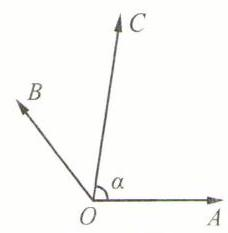
\includegraphics[width=0.2\textwidth]{bodyxb/src/bo_d20aucref24c73anc48g_14_1276_1896_228_233_0.jpg}
\end{center}


(第 97 题)

98. 在梯形 ${ABCD}$ 中, ${AB}//{CD},M,N$ 分别是 ${AD},{BC}$ 的中点,且 $\dfrac{CD}{AB} = k\left( {k \neq  1}\right)$ . 设 $\vv{AD} = a$ , $\vv{AB} = \vv{b}$ ,试用 $\vv{a},\vv{b}$ 表示 $\vv{DC},\vv{BC},\vv{MN}$ .

99. 在 ▱ ${ABCD}$ 中, $\vv{AC} = \vv{a},\vv{BD} = \vv{b}$ ,试用 $\vv{a},\vv{b}$ 表示 $\vv{AB},\vv{BC}$ .

100. 在 $\bigtriangleup  {ABC}$ 中, ${AM} = \dfrac{1}{3}{AB}$ , ${AN} = \dfrac{1}{4}{AC}$ ,线段 ${BN}$ 与 ${CM}$ 交于点 $P$ ,求证: $\vv{AP} = \dfrac{3}{11}\vv{AB} +$  $\dfrac{2}{11}\vv{AC}$

101. 已知 $G$ 是 $\bigtriangleup {ABC}$ 的重心,过 $G$ 作直线 ${MN}$ ,与 ${AB},{AC}$ 两边分别交于 $M,N$ 两点,且 $\vv{AM} = x\vv{AB},\vv{AN} = y\vv{AC}$ ,求 $\dfrac{xy}{x + y}$ 的值.

102. 平面上给定 $\bigtriangleup {ABC}$ 及点 $O$ ,对平面上任意点 $P$ ,证明: 存在唯一的实数 $x,y,z$ ,使得 $x + y$  $+ z = 1$ ,且 $\vv{OP} = x\vv{OA} + y\vv{OB} + z\vv{OC}$ .

\section*{(B)}

103. 若两个向量 $\vv{a},\vv{b}$ 不共线,且 $x\left( {\vv{a} + \vv{b}}\right)  + y\left( {\vv{a} - \vv{b}}\right)  = 2\vv{a} + 4\vv{b}$ ,则实数 $x,y$ 的值分别为(   )

(A) $3, - 1$ . (B)-3,1. (C) $- 3, - 1$ . (D)3,1.

104. 已知两个向量 ${\vv{e}}_{1},{\vv{e}}_{2}$ 不共线,且 $\vv{a} = {2\lambda }{\vv{e}}_{1} + {\vv{e}}_{2},\vv{b} = \left( {3{\lambda }^{2} - 1}\right) {\vv{e}}_{1} + \left( {6 - {5\lambda }}\right) {\vv{e}}_{2}$ . 若 $\vv{a} = \vv{b}$ ,则实数 $\lambda$ 的值为 (   )

(A) $- \dfrac{1}{3}$ . (B) $\dfrac{1}{3}$ . (C) -1 . (D) 1 .

105. 已知 $\left| \vv{OA}\right|  = 1,\left| \vv{OB}\right|  = \sqrt{3},\vv{OA} \cdot  \vv{OB} = 0$ ,点 $C$ 在 $\angle {AOB}$ 内,且 $\angle {AOC} = {30}^{ \circ  }$ . 若 $\vv{OC}$  $= m\vv{OA} + n\vv{OB}\left( {m,n \in  \mathbf{R}}\right)$ ,则 $\dfrac{m}{n}$ 等于(   )

(A) $\dfrac{1}{3}$ . (B) 3. (C) $\dfrac{\sqrt{3}}{3}$ . (C) $\sqrt{3}$ .

106. 已知 $\vv{OA} = \vv{a},\vv{OB} = \vv{b},C$ 为线段 ${AB}$ 上距点 $A$ 较近的一个三等分点, $D$ 为线段 ${CB}$ 上距点 $C$ 较近的一个三等分点,则用 $a,b$ 表示 $\vv{OD}$ 为(   )

(A) $\dfrac{1}{9}\left( {4\vv{a} + 5\vv{b}}\right)$ . (B) $\dfrac{1}{16}\left( {9\vv{a} + 7\vv{b}}\right)$ . (C) $\dfrac{1}{3}\left( {2\vv{a} + \vv{b}}\right)$ . (D) $\dfrac{1}{4}\left( {3\vv{a} + \vv{b}}\right)$ .

107. 设 $a$ 是已知的平面向量且 $a \neq  0$ ,关于向量 $a$ 的分解,有如下四个命题:

① 给定向量 $\vv{b}$ ,总存在向量 $\vv{c}$ ,使 $\vv{a} = \vv{b} + \vv{c}$ ；

②给定不平行向量 $\vv{b}$ 和 $\vv{c}$ ,总存在实数 $\lambda$ 和 $\mu$ ,使 $\vv{a} = \lambda \vv{b} + \mu \vv{c}$ ；

③给定单位向量 $\vv{b}$ 和正数 $\mu$ ,总存在单位向量 $c$ 和实数 $\lambda$ ,使 $\vv{a} = \lambda \vv{b} + \mu \vv{c}$ ；

④给定正数 $\lambda$ 和 $\mu$ ,总存在单位向量 $\vv{b}$ 和单位向量 $c$ ,使 $\vv{a} = \lambda \vv{b} + \mu \vv{c}$ ；

上述命题中的向量 $b,c$ 和 $a$ 在同一平面内且两两不共线,则真命题的个数是 (   )

(A) 1 . (B) 2 . (C) 3 . (D) 4 .

108. 给出下列命题:①若 $a,b$ 共线,且 $\left| \vv{a}\right|  = \left| \vv{b}\right|$ ,则 $\left( {\vv{a} - \vv{b}}\right) //\left( {\vv{a} + \vv{b}}\right)$ ；②若 $\vv{a} = 2\vv{e},\vv{b} = 3\vv{e}$ , 则 $\vv{a} = \dfrac{3}{2}\vv{b}$ ；③ 若 $\vv{a} = {\vv{e}}_{1} - {\vv{e}}_{2},\vv{b} =  - 3{\vv{e}}_{1} + 3{\vv{e}}_{2}$ ,且 ${\vv{e}}_{1} \neq  {\vv{e}}_{2}$ ,则 $\left| \vv{a}\right|  = 3\left| \vv{b}\right|$ ；④ 在 $\bigtriangleup  {ABC}$ 中, ${AD}$ 是边 ${BC}$ 上的中线,则 $\vv{AB} + \vv{AC} = 2\vv{AD}$ . 其中真命题是\blkda{}(填序号).

109. 如图,两块斜边长相等的直角三角板拼在一起,若 $\vv{AD} = x\vv{AB} + y\vv{AC}$ ,则 $x =$ \blkda{}, $y =$ \blkda{}.

\begin{center}
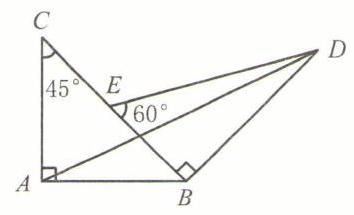
\includegraphics[width=0.3\textwidth]{bodyxb/src/bo_d20aucref24c73anc48g_16_1161_353_354_215_0.jpg}
\end{center}


(第 109 题)

110. 设 $I$ 为 $\bigtriangleup {ABC}$ 的内心. 当 ${AB} = {AC} = 5,{BC} = 6$ 时, $\vv{AI} = x\vv{AB} + y\vv{BC}$ ,则实数 $x,y$ 的值分别为\blkda{}.

111. 如图, ${OM}//{AB}$ ,点 $P$ 在由射线 ${OM}$ 、线段 ${OB}$ 及 ${AB}$ 的延长线围成的区域内 (不含边界) 运动,且 $\vv{OP} = x\vv{OA} + y\vv{OB}$ ,则实数 $x$ 的取值范围是\blkda{}；当 $x =  - \dfrac{1}{2}$ 时,实数 $y$ 的取值范围是\blkda{}.

\begin{center}
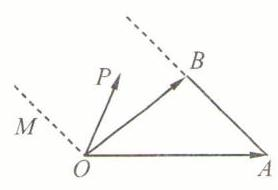
\includegraphics[width=0.2\textwidth]{bodyxb/src/bo_d20aucref24c73anc48g_16_1211_701_278_190_0.jpg}
\end{center}


(第 111 题)

112. 已知 $\vv{OA} = \vv{a},\vv{OB} = \vv{b}$ ,且 $\left| {OA}\right|  = \left| {OB}\right|  = 1,\angle {AOB} = {120}^{ \circ  }$ ,又 $\left| {OC}\right|  =$ 5,且 ${OC}$ 平分 $\angle {AOB}$ . 若 $\vv{OC} = \lambda \vv{a} + \mu \vv{b}$ ,则 $\lambda  =$ \blkda{}, $\mu  =$ \blkda{}.

113. 若 $\bigtriangleup {ABC}$ 的外接圆的圆心为 $O$ ,两条边上的高的交点为 $H,\vv{OH} = m\left( {\vv{OA} + \vv{OB} + \vv{OC}}\right)$ , 则实数 $m =$ \blkda{}.

114. 已知 $G$ 为 $\bigtriangleup {ABC}$ 的重心, $\vv{AB} = \vv{a},\vv{AC} = \vv{b}$ ,试用 $\vv{a},\vv{b}$ 表示 $\vv{AG}$ .

115. 已知 $\vv{a},\vv{b}$ 是同一平面上的两个不共线的向量, ${\lambda }_{1},{\lambda }_{2},{\mu }_{1},{\mu }_{2} \in  \mathbf{R}$ ,求证: $\vv{c} = {\lambda }_{1}\vv{a} + {\mu }_{1}\vv{b}$ 和 $\vv{d}$  $= {\lambda }_{2}\vv{a} + {\mu }_{2}\vv{b}$ 为共线向量的充要条件是 ${\lambda }_{1}{\mu }_{2} = {\lambda }_{2}{\mu }_{1}$ .

116. 如图, $A,B,C$ 三点不共线,且 $\vv{OA} = \vv{a},\vv{OB} = \vv{b},\vv{OC} = \vv{c}$ . 若 $\left| \vv{a}\right|  = 1$ , $\left| \vv{b}\right|  = 2,\left| \vv{c}\right|  = 3$ ,且 $\angle {AOB} = {90}^{ \circ  },\angle {AOC} = {120}^{ \circ  }$ ,试用 $\vv{a},\vv{b}$ 表示 $\vv{c}$ .

\begin{center}
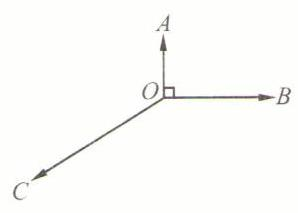
\includegraphics[width=0.2\textwidth]{bodyxb/src/bo_d20aucref24c73anc48g_16_1193_1310_298_213_0.jpg}
\end{center}


(第 116 题)

117. 如图,在 $\bigtriangleup {AOB}$ 中, $\vv{OC} = \dfrac{1}{4}\vv{OA},\vv{OD} = \dfrac{1}{2}\vv{OB},{AD}$ 与 ${BC}$ 交于点 $M$ . 设 $\vv{OA} = \vv{a},\vv{OB} = \vv{b}$ .

(1)试用 $a,b$ 表示 $\vv{OM}$ ；

\begin{center}
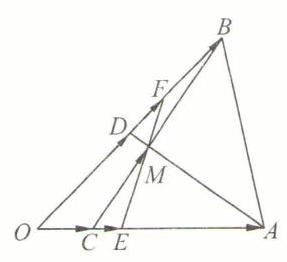
\includegraphics[width=0.2\textwidth]{bodyxb/src/bo_d20aucref24c73anc48g_16_1207_1631_287_262_0.jpg}
\end{center}


(第 117 题)

(2)在线段 ${AC}$ 上取一点 $E$ ,线段 ${BD}$ 上取一点 $F$ ,使 ${EF}$ 过点 $M$ , 设 $\vv{OE} = \lambda \vv{OA},\vv{OF} = \mu \vv{OB}$ ,求证: $\dfrac{1}{7\lambda } + \dfrac{3}{7\mu } = 1$ .

118. 设 $O$ 为 $\bigtriangleup {ABC}$ 内一点,记 $\alpha  = \dfrac{{S}_{\bigtriangleup {BOC}}}{{S}_{\bigtriangleup {ABC}}},\beta  = \dfrac{{S}_{\bigtriangleup {COA}}}{{S}_{\bigtriangleup {ABC}}},\gamma  = \dfrac{{S}_{\bigtriangleup {AOB}}}{{S}_{\bigtriangleup {ABC}}}$ . 求证: $\alpha \vv{OA} + \beta \vv{OB} + \gamma \vv{OC} = \vv{0}$ .

\section*{四、向量的坐标表示}

\section*{【典型例题和解题技巧】}

1. 按运算法则进行向量的坐标运算.

若向量 $\vv{a} = \left( {{x}_{1},{y}_{1}}\right) ,\vv{b} = \left( {{x}_{2},{y}_{2}}\right)$ ,则有:

(1) $\vv{a} + \vv{b} = \left( {{x}_{1} + {x}_{2},{y}_{1} + {y}_{2}}\right)$ ;

(2) $\vv{a} - \vv{b} = \left( {{x}_{1} - {x}_{2},{y}_{1} - {y}_{2}}\right)$ ;

(3) $\lambda \vv{a} = \left( {\lambda {x}_{1},\lambda {y}_{1}}\right)$ ;

(4) $\vv{a} \cdot  \vv{b} = {x}_{1}{x}_{2} + {y}_{1}{y}_{2}$ .

例 1 (1) 已知向量 $\vv{a} = \left( {-1,2}\right) ,\vv{b} = \left( {2,1}\right)$ ,求 $2\vv{a} + 3\vv{b},\vv{a} - 3\vv{b},\dfrac{1}{2}\vv{a} - \dfrac{1}{3}\vv{b}$ ；

(2)已知点 $A\left( {4,6}\right)$ , $B\left( {7,5}\right)$ , $C\left( {1,8}\right)$ ,求 $\vv{AB} - \dfrac{1}{2}\vv{AC}$ .

解 (1) ${2a} + {3b} = 2\left( {-1,2}\right)  + 3\left( {2,1}\right)  = \left( {-2 + 6,4 + 3}\right)  = \left( {4,7}\right)$ ,

$\vv{a} - 3\vv{b} = \left( {-1,2}\right)  - 3\left( {2,1}\right)  = \left( {-1 - 6,2 - 3}\right)  = \left( {-7, - 1}\right)$ ,

$\dfrac{1}{2}\vv{a} - \dfrac{1}{3}\vv{b} = \dfrac{1}{2}\left( {-1,2}\right)  - \dfrac{1}{3}\left( {2,1}\right)  = \left( {-\dfrac{1}{2} - \dfrac{2}{3},1 - \dfrac{1}{3}}\right)  = \left( {-\dfrac{7}{6},\dfrac{2}{3}}\right) .$

(2) $\vv{AB} - \dfrac{1}{2}\vv{AC} = \left( {7,5}\right)  - \left( {4,6}\right)  - \dfrac{1}{2}\left\lbrack  {\left( {1,8}\right)  - \left( {4,6}\right) }\right\rbrack   = \left( {3, - 1}\right)  - \dfrac{1}{2}\left( {-3,2}\right)  = \left( {\dfrac{9}{2}, - 2}\right)$ .

例 2 已知点 $O\left( {0,0}\right) ,A\left( {1,2}\right) ,B\left( {4,5}\right)$ ,且 $\vv{OP} = \vv{OA} + t\vv{AB}\left( {t \in  \mathbf{R}}\right)$ .

(1)当 $t$ 为何值时,点 $P$ 在 $x$ 轴上? 点 $P$ 在二、四象限角平分线上? 点 $P$ 在第二象限?

(2)四边形 ${OABP}$ 能否成为平行四边形？若能,求出相应的 $t$ 的值；若不能,请说明理由.

解(1)向量 $\vv{OP} = \left( {1 + {3t},2 + {3t}}\right)$ .

若点 $P$ 在 $x$ 轴上,则只需 $2 + {3t} = 0$ ,得 $t =  - \dfrac{2}{3}$ ;

若点 $P$ 在二、四象限角平分线上,则只需 $1 + {3t} =  - \left( {2 + {3t}}\right)$ ,得 $t =  - \dfrac{1}{2}$ ;

若点 $P$ 在第二象限,则只需 $\left\{  \begin{array}{l} 1 + {3t} < 0, \\  2 + {3t} > 0, \end{array}\right.$ 得 $- \dfrac{2}{3} < t <  - \dfrac{1}{3}$ .

(2)向量 $\vv{OA} = \left( {1,2}\right) ,\vv{PB} = \left( {3 - {3t},3 - {3t}}\right)$ .

若 ${OABP}$ 为平行四边形,则 $\vv{OA} = \vv{PB}$ .

$\therefore \left\{  \begin{array}{l} 3 - {3t} = 1, \\  3 - {3t} = 2, \end{array}\right.$ 此方程组无解,所以四边形 ${OABP}$ 不能成为平行四边形.

2. 模与单位向量.

若向量 $\vv{a} = \left( {x,y}\right)$ ,则 $\left| \vv{a}\right|  = \sqrt{{x}^{2} + {y}^{2}},\vv{a}$ 的单位向量 ${\vv{a}}_{0} = \dfrac{\vv{a}}{\left| \vv{a}\right| }$ .

例 3 已知向量 $a = \left( {-6,8}\right)$ . 求:

(1)向量 $\vv{a}$ 的模； (2)向量 $\vv{a}$ 的单位向量 ${\vv{a}}_{0}$ .

解(1) $\left| \vv{a}\right|  = \sqrt{{\left( -6\right) }^{2} + {8}^{2}} = {10}$ .

(2) ${\vv{a}}_{0} = \dfrac{\vv{a}}{\left| \vv{a}\right| } = \dfrac{\left( -6,8\right) }{10} = \left( {-\dfrac{3}{5},\dfrac{4}{5}}\right)$ .

3. 向量的平行、垂直.

若向量 $\vv{a} = \left( {{x}_{1},{y}_{1}}\right) ,\vv{b} = \left( {{x}_{2},{y}_{2}}\right)$ ,则 $\vv{a}//\vv{b} \Leftrightarrow  {x}_{1}{y}_{2} = {x}_{2}{y}_{1}$ .

若向量 $\vv{a} = \left( {{x}_{1},{y}_{1}}\right) ,\vv{b} = \left( {{x}_{2},{y}_{2}}\right)$ ,则有 $\vv{a} \bot  \vv{b} \Leftrightarrow  {x}_{1}{x}_{2} + {y}_{1}{y}_{2} = 0$ .

例 4 已知 $O$ 为坐标原点,在 $\bigtriangleup {ABC}$ 中,向量 $\vv{OA} = \left( {2, - 3}\right) ,\vv{OB} = \left( {1,4}\right)$ ,且 $\vv{OC} = 3\vv{OA}$ , $\vv{OD} = 3\vv{OB},\vv{OE} = 2\vv{OA} + \vv{OB}$ ,求 $C,D,E$ 三点的坐标,并判断 $C,D,E$ 三点是否共线.

解 $\because \vv{OC} = 3\vv{OA} = 3\left( {2, - 3}\right)  = \left( {6, - 9}\right) ,\vv{OD} = 3\vv{OB} = 3\left( {1,4}\right)  = \left( {3,{12}}\right)$ ,

$\vv{OE} = 2\vv{OA} + \vv{OB} = \left( {4, - 6}\right)  + \left( {1,4}\right)  = \left( {5, - 2}\right)$ ,

又 $\because \vv{OC},\vv{OD},\vv{OE}$ 的起点均在原点,

$\therefore C,D,E$ 三点的坐标分别为 $\left( {6, - 9}\right) ,\left( {3,{12}}\right) ,\left( {5, - 2}\right)$ .

$\because \vv{CE} = \vv{OE} - \vv{OC} = \left( {5, - 2}\right)  - \left( {6, - 9}\right)  = \left( {-1,7}\right)$ ,

$\vv{CD} = \vv{OD} - \vv{OC} = \left( {3,{12}}\right)  - \left( {6, - 9}\right)  = \left( {-3,{21}}\right)  = 3\left( {-1,7}\right)  = 3\vv{CE}$ ,

$\therefore \vv{CE}//\vv{CD}$ ,且 $\vv{CE},\vv{CD}$ 有公共点 $C,\therefore C,D,E$ 三点共线.

例 5 在 $\mathrm{{Rt}}\bigtriangleup {ABC}$ 中,向量 $\vv{AB} = \left( {2,3}\right) ,\vv{AC} = \left( {1,k}\right)$ ,求实数 $k$ 的值.

解 分下列三种情况讨论:

(1)当 $\angle A = {90}^{ \circ  }$ 时, $\because \vv{AB} \cdot  \vv{AC} = 0,\therefore 2 \times  1 + {3k} = 0,\therefore k =  - \dfrac{2}{3}$ .

(2)当 $\angle B = {90}^{ \circ  }$ 时, $\vv{BC} = \vv{AC} - \vv{AB} = \left( {-1,k - 3}\right)$ .

$\because \vv{AB} \cdot  \vv{BC} = 0,\therefore 2 \times  \left( {-1}\right)  + 3\left( {k - 3}\right)  = 0,\therefore k = \dfrac{11}{3}.$

(3) 当 $\angle C = {90}^{ \circ  }$ 时, $\because \vv{AC} \cdot  \vv{BC} = 0,\therefore  - 1 + k\left( {k - 3}\right)  = 0,\therefore k = \dfrac{3 \pm  \sqrt{13}}{2}$ .

综上所述, $k =  - \dfrac{2}{3}$ 或 $\dfrac{11}{3}$ 或 $\dfrac{3 \pm  \sqrt{13}}{2}$ .

例 6 已知点 $A\left( {x,1}\right) ,B\left( {{2x},2}\right) ,C\left( {1,{2x}}\right) ,D\left( {5,{3x}}\right)$ . 当 $x$ 为何值时,向量 $\vv{AB}$ 与 $\vv{CD}$ 共线且方向相同？此时,点 $A,B,C,D$ 是否在同一条直线上?

解 $\because \vv{AB} = \left( {x,1}\right) ,\vv{CD} = \left( {4,x}\right) ,\vv{AB}//\vv{CD} \Leftrightarrow  {x}^{2} - 4 = 0,\therefore x =  \pm  2$ .

当 $x = 2$ 时, $\vv{AB} = \left( {2,1}\right) ,\vv{CD} = \left( {4,2}\right)  \Rightarrow  \vv{CD} = 2\vv{AB}$ ;

当 $x =  - 2$ 时, $\vv{AB} = \left( {-2,1}\right) ,\vv{CD} = \left( {4, - 2}\right)  \Rightarrow  \vv{CD} =  - 2\vv{AB}$ .

故当 $x = 2$ 时, $\vv{AB}$ 与 $\vv{CD}$ 共线且方向相同.

此时, $\vv{BD} = \left( {5 - {2x},{3x} - 2}\right)  = \left( {1,4}\right) .\because 2 \times  4 - 1 \times  1 \neq  0,\therefore \vv{AB}$ 与 $\vv{BD}$ 不共线,

故点 $A,B,C,D$ 不在同一条直线上.

4. 线段的定比分点的坐标公式.

设点 ${P}_{1}\left( {{x}_{1},{y}_{1}}\right) ,{P}_{2}\left( {{x}_{2},{y}_{2}}\right) ,P\left( {x,y}\right)$ 是直线 ${P}_{1}{P}_{2}$ 上一点,且 $\vv{{P}_{1}P} = \lambda \vv{P{P}_{2}}$ ,

则有 $\left\{  \begin{array}{l} x = \dfrac{{x}_{1} + \lambda {x}_{2}}{1 + \lambda }, \\  y = \dfrac{{y}_{1} + \lambda {y}_{2}}{1 + \lambda }. \end{array}\right.$

例 7 经过点 $M\left( {-2,3}\right)$ 的直线分别与 $x$ 轴、 $y$ 轴交于 $A,B$ 两点,且 $\left| \vv{AB}\right|  = 3\left| \vv{AM}\right|$ ,求点 $A,B$ 的坐标.

解 设点 $A\left( {a,0}\right) ,B\left( {0,b}\right)$ .

由 $\left| \vv{AB}\right|  = 3\left| \vv{AM}\right|$ ,得 $\vv{AB} = 3\vv{AM}$ 或 $\vv{AB} =  - 3\vv{AM}$ .

当 $\vv{AB} = 3\vv{AM}$ 时,有 $\vv{BM} = 2\vv{MA}$ ,

$\therefore  - 2 = \dfrac{0 + {2a}}{1 + 2},3 = \dfrac{b + 2 \times  0}{1 + 2}$ ,得 $a =  - 3,b = 9$ ;

当 $\vv{AB} =  - 3\vv{AM}$ 时,有 $\vv{BM} =  - 4\vv{MA},\therefore  - 2 = \dfrac{0 - {4a}}{1 - 4},3 = \dfrac{b - 4 \times  0}{1 - 4}$ ,得 $a =  - \dfrac{3}{2},b =  - 9$ .

$\therefore$ 点 $A,B$ 的坐标分别为 $\left( {-3,0}\right) ,\left( {0,9}\right)$ 或 $\left( {-\dfrac{3}{2},0}\right) ,\left( {0, - 9}\right)$ .

注意(1)运用定比分点的坐标公式时要分清 (或选定) 起点、终点及分点,从而确定 $\lambda$ .

(2) $\left| \vv{AB}\right|  = 3\left| \vv{AM}\right|$ 表示向量的模的关系,当 $A,B,M$ 三点共线时, $\left| \vv{AB}\right|  = 3\left| \vv{AM}\right|  \Leftrightarrow  \vv{AB}$  $=  \pm  3\vv{AM}$ .

\section*{【训练题】}

\section*{(A)}

119. 若向量 $\vv{a}$ 的起点坐标为(3,1),终点坐标为(-1, - 3),则向量 $\vv{a}$ 的坐标为 (   )

(A)(-1, - 3). (B)(4,4). (C)(-4, - 2). (D)(-4, - 4).

120. 若向量 $\vv{AB} = \left( {6,1}\right) ,\vv{BC} = \left( {-1,2}\right) ,\vv{CD} = \left( {2, - 3}\right)$ ,则向量 $\vv{AD}$ 的坐标为(   )

(A)(5,2). (B)(7,0). (C)(-7,0). (D)(5, - 4).

121. 若向量 $\vv{a} = \left( {1,1}\right) ,\vv{b} = \left( {1, - 1}\right) ,\vv{c} = \left( {-2,4}\right)$ ,则 $\vv{c}$ 等于(   )

(A) $- \vv{a} + 3\vv{b}$ . (B) $\vv{a} - 3\vv{b}$ . (C) ${3a} - b$ . (D) $- 3\vv{a} + \vv{b}$ .

122. 若 $P\left( {3, - 6}\right) ,Q\left( {-5,2}\right) ,R\left( {m, - 9}\right)$ 三点共线,则实数 $m$ 的值为 (   )

(A) -9. (B) -6. (C) 9. (D) 6.

123. 若向量 $\vv{AB} = \left( {3, - 1}\right) ,\vv{ON} = \left( {-2,0}\right)$ ,且 $\vv{AB} = \vv{MN}$ ,则向量 $\vv{OM}$ 的坐标为(   )

(A)(1, - 1). (B)(5, - 1). (C)(-5,1). (D)(1, - 5).

124. 设 $i,j$ 分别是 $x$ 轴, $y$ 轴正方向上的单位向量, $O$ 为坐标原点. 若 $\vv{OA} = {4i} + {2j},\vv{OB} = {3i} +$  ${4j}$ ,则 $2\vv{OA} + \vv{OB}$ 的坐标为(   )

(A)(1, - 2). (B)(7,6). (C)(5,0). (D)(11,8).

125. 已知向量 $\vv{a} = \left( {{\cos }^{7}{5}^{ \circ  },{\sin }^{7}{5}^{ \circ  }}\right) ,\vv{b} = \left( {{\cos }^{1}{5}^{ \circ  },{\sin }^{1}{5}^{ \circ  }}\right)$ ,那么 $\left| {\vv{a} - \vv{b}}\right|$ 的值为 (   )

(A) $\dfrac{1}{2}$ . (B) $\dfrac{\sqrt{2}}{2}$ . (C) $\dfrac{\sqrt{3}}{2}$ . (D) 1 .

126. 若向量 $\vv{a} = \left( {3,2}\right) ,\vv{b} = \left( {x,4}\right)$ ,且 $\vv{a}//\vv{b}$ ,则 $x$ 的值为(   )

(A) 6. (B) -6. (C) $\dfrac{8}{3}$ . (D) $- \dfrac{8}{3}$ .

127. 若 $a,b$ 是一组基底,向量 $c = {xa} + {yb}\left( {x,y \in  \mathbf{R}}\right)$ ,则称(x, y)为向量 $c$ 在基底 $a,b$ 下的坐标. 现已知向量 $\vv{c}$ 在基底 $\vv{a} = \left( {1, - 1}\right) ,\vv{b} = \left( {2,1}\right)$ 下的坐标为(-2,2),则 $\vv{c}$ 在另一组基底 $\vv{m} = \left( {-1,1}\right) ,\vv{n} = \left( {1,2}\right)$ 下的坐标为 (   )

(A)(2,0). (B)(0, - 2). (C)(-2,0). (D)(0,2).

128. 若向量 $\vv{a} = \left( {\dfrac{3}{2},\sin \alpha }\right) ,\vv{b} = \left( {\cos \alpha ,\dfrac{1}{3}}\right)$ ,且 $\vv{a}//\vv{b}$ ,则锐角 $\alpha$ 为(   )

(A) ${30}^{ \circ  }$ . (B) ${60}^{ \circ  }$ . (C) ${45}^{ \circ  }$ . (D) ${75}^{ \circ  }$ .

129. 若点 $P\left( {-1, - 1}\right) ,Q\left( {2,5}\right)$ ,点 $R$ 在直线 ${PQ}$ 上,且 $\vv{PR} =  - 5\vv{QR}$ ,则点 $R$ 的坐标为(   )

(A) $\left( {\dfrac{11}{4},\dfrac{13}{2}}\right)$ . (B) $\left( {\dfrac{11}{4},\dfrac{3}{2}}\right)$ . (C) $\left( {\dfrac{3}{2},\dfrac{13}{2}}\right)$ . (D) $\left( {\dfrac{3}{2},4}\right)$ .

130. 当 $\vv{AP} = \dfrac{1}{3}\vv{PB}$ 时,有 $\vv{PB} = \lambda \vv{BA}$ ,则实数 $\lambda$ 的值为 (   )

(A) $\dfrac{3}{4}$ . (B) $\dfrac{4}{3}$ . (C) $- \dfrac{4}{3}$ . (D) $- \dfrac{3}{4}$ .

131. 若过 ${P}_{1}\left( {-1,2}\right) ,{P}_{2}\left( {5,6}\right)$ 两点的直线与 $x$ 轴交于点 $P$ ,设 $\vv{{P}_{1}P} = \lambda \vv{P{P}_{2}}$ ,则 $\lambda$ 的值为(   )

(A) $- \dfrac{1}{3}$ . (B) $- \dfrac{1}{5}$ . (C) $\dfrac{1}{5}$ . (D) $\dfrac{1}{3}$ .

132. 若向量 $\vv{b}$ 与 $\vv{a} = \left( {1, - 2}\right)$ 的夹角为 ${180}^{ \circ  }$ ,且 $\left| \vv{b}\right|  = 3\sqrt{5}$ ,则 $\vv{b}$ 等于(   )

(A)(-3,6). (B)(3, - 6). (C)(6, - 3). (D)(-6,3).

133. 若向量 $\vv{a} = \left( {3, - 1}\right) ,\vv{b} = \left( {1, - 2}\right)$ ,则 $\vv{a}$ 与 $\vv{b}$ 的夹角为(   )

(A) $\dfrac{\pi }{6}$ . (B) $\dfrac{\pi }{4}$ . (C) $\dfrac{\pi }{3}$ . (D) $\dfrac{\pi }{2}$ .

134. 在 $\bigtriangleup {ABC}$ 中, $\angle C = {90}^{ \circ  }$ ,向量 $\vv{AB} = \left( {k,1}\right) ,\vv{AC} = \left( {2,3}\right)$ ,则实数 $k$ 的值是(   )

(A) 5 . (B) -5 . (C) $\dfrac{3}{2}$ . (D) $- \dfrac{3}{2}$ .

135. 已知点 $A\left( {3,1}\right) ,B\left( {6,1}\right) ,C\left( {4,3}\right) ,D$ 为线段 ${BC}$ 的中点,那么向量 $\vv{AC}$ 与 $\vv{DA}$ 夹角的余弦值为(   )

(A) $- \dfrac{4}{5}$ . (B) $\dfrac{4}{5}$ . (C) $- \dfrac{3}{5}$ . (D) $\dfrac{3}{5}$ .

136. 若向量 $\vv{a} = \left( {\cos \theta ,\sin \theta }\right) ,\vv{b} = \left( {\sqrt{3}, - 1}\right)$ ,则 $\left| {2\vv{a} - \vv{b}}\right|$ 的最大值、最小值分别为(   )

(A) $4\sqrt{2},0$ . (B) $4,2\sqrt{2}$ . (C)10,0. (D)4,0.

137. 已知向量 $\vv{a} = \left( {1,2}\right) ,\vv{b} = \left( {-2, - 4}\right) ,\left| \vv{c}\right|  = \sqrt{5}$ . 若 $\left( {\vv{a} + \vv{b}}\right)  \cdot  \vv{c} = \dfrac{5}{2}$ ,则 $\vv{a}$ 与 $\vv{c}$ 的夹角为(   )

(A) ${30}^{ \circ  }$ . (B) ${60}^{ \circ  }$ . (C) ${120}^{ \circ  }$ . (D) ${150}^{ \circ  }$ .

138. 若向量 $\vv{a} = \left( {2,3}\right) ,\vv{b} = \left( {-4,7}\right)$ ,则 $\vv{a}$ 在 $\vv{b}$ 方向上的数量投影为(   )

(A) $\sqrt{13}$ . (B) $\dfrac{\sqrt{13}}{5}$ . (C) $\dfrac{\sqrt{65}}{5}$ . (D) $\sqrt{65}$ .

139. 已知点 $O\left( {0,0}\right) ,A\left( {3,0}\right) ,B\left( {0,3}\right)$ ,点 $P$ 在线段 ${AB}$ 上. 若 $\vv{AP} = t\vv{AB}\left( {0 \leq  t \leq  1}\right)$ ,则 $\vv{OA} \cdot  \vv{OP}$ 的最大值为(   )

(A) 3. (B) 6. (C) 9. (D) 12 .

140. 若向量 $\vv{a} + \vv{b} = \left( {-3, - 4}\right) ,\vv{a} - \vv{b} = \left( {5,2}\right)$ ,则向量 $\vv{a} =$ \blkda{}, $\vv{b} =$ \blkda{}.

141. 已知 $\left| \vv{a}\right|  = 5,\vv{b} = \left( {1,2}\right) ,\vv{a}//\vv{b}$ ,且方向相反,则向量 $\vv{a} =$ \blkda{}.

142. 已知 $O$ 为坐标原点,若向量 $a$ 以线段 ${OB}$ 的中点 $A\left( {-2,1}\right)$ 为起点,且 $a = \left( {3,2}\right)$ ,则以点 $B$ 为起点的向量 ${2a}$ 的终点坐标为\blkda{}.

143. 已知向量 $\vv{a} = \left( {1,2}\right) ,\vv{b} = \left( {2,3}\right)$ . 若向量 $\lambda \vv{a} + \vv{b}$ 与向量 $\vv{c} = \left( {-4, - 7}\right)$ 共线,则 $\lambda$  $=$ \blkda{}.

144. 与向量 $\vv{a} = \left( {3, - 4}\right)$ 平行的单位向量是\blkda{}.

145. 已知向量 $\vv{a} = \left( {3, - 2}\right) ,\vv{b} = \left( {-2,1}\right) ,\vv{c} = \left( {7, - 4}\right)$ . 若 $\vv{c} = \mathbf{\lambda }\vv{a} + \mathbf{\mu }\vv{b}$ ,则 $\mathbf{\lambda } =$ \blkda{}, $\mathbf{\mu } =$ \blkda{}.

146. 若向量 $\vv{a} = \left( {x,2}\right) ,\vv{b} = \left( {-4,y}\right) ,\vv{c} = \left( {-3, - 5}\right)$ ,且 $\vv{c} =  - \dfrac{1}{2}\vv{a} + \dfrac{3}{2}\vv{b}$ ,则实数 $x =$ \blkda{}, $y =$ \blkda{}.

147. 若两个不相等的向量 $\vv{a} = \left( {\dfrac{1}{2},\cos \alpha }\right) ,\vv{b} = \left( {\sin \alpha , - \dfrac{\sqrt{3}}{2}}\right)$ ,满足 $\vv{a}//\vv{b},\alpha$ 为钝角,则 $\alpha$  $=$ \blkda{}.

148. 若向量 $\vv{a} = \left( {1,\sin \theta }\right) ,\vv{b} = \left( {1,\cos \theta }\right)$ ,则 $\left| {\vv{a} - \vv{b}}\right|$ 的最大值为\blkda{}.

149. 若三角形的两个顶点为 $A\left( {-{10},3}\right) ,B\left( {6, - 4}\right)$ ,三角形的重心为 $M\left( {-2,3}\right)$ ,则三角形的另一个顶点 $C$ 的坐标为\blkda{}.

150. 已知向量 $a = \left( {-4,2}\right)$ 的终点在原点,求向量 $a$ 的起点坐标.

151. 在平面直角坐标系中, $O$ 为坐标原点,已知两点 $A\left( {3,1}\right) ,B\left( {-1,3}\right)$ . 若点 $C$ 满足 $\vv{OC} =$  $\alpha \vv{OA} + \beta \vv{OB},\alpha ,\beta  \in  \mathbf{R}$ ,且 $\alpha  + \beta  = 1$ ,求点 $C$ 的轨迹方程.

152. 已知 $A,B,C,D$ 为坐标平面上的四个点, $\vv{AB} = \vv{CD}$ ,点 $A$ 的坐标为(3,1),点 $B$ 的坐标为 (-2, - 2).

(1)若点 $C$ 的坐标为(-1,4),求点 $D$ 的坐标；

(2)若坐标原点为 $O,\vv{OP} = \vv{AB}$ ,求点 $P$ 的坐标.

153. 已知 $O$ 为坐标原点,向量 $\vv{OA} = \left( {-2,m}\right) ,\vv{OB} = \left( {n,1}\right) ,\vv{OC} = \left( {5, - 1}\right)$ . 若 $A,B,C$ 三点共线,且 $m = {2n}$ ,求实数 $m,n$ 的值.

154. 给定两个向量 $\vv{a} = \left( {3,4}\right) ,\vv{b} = \left( {2, - 1}\right)$ ,求 $\vv{a} + x\vv{b}$ 与 $\vv{a} - \vv{b}$ 平行时实数 $x$ 的值.

155. 已知向量 $a = \left( {8,2}\right) ,b = \left( {3,3}\right) ,c = \left( {6,{12}}\right) ,p = \left( {6,4}\right)$ . 问: 是否存在实数 $x,y,z$ 同时满足下列两个条件: (1) $p = {xa} + {yb} + {zc};\left( 2\right) x + y + z = 1$ ? 若存在,请求出 $x,y,z$ 的值; 若不存在, 请说明理由.

156. 已知点 $A\left( {3,0}\right) ,B\left( {-1, - 6}\right) ,P$ 是直线 ${AB}$ 上一点,且 $\left| \vv{AP}\right|  = \dfrac{1}{3}\left| \vv{AB}\right|$ ,求点 $P$ 的坐标.

157. 已知向量 $c = {ma} + {nb} = \left( {-2\sqrt{3},2}\right) ,a \bot  c,b$ 与 $c$ 的夹角为 ${120}^{ \circ  }$ ,且 $b \cdot  c =  - 4,\left| a\right|  =$  $2\sqrt{2}$ ,求实数 $m,n$ 的值及 $\vv{a}$ 与 $\vv{b}$ 的夹角.

\section*{(B)}

158. 在 ▱ ${ABCD}$ 中,若 $\vv{AB} = \left( {2,4}\right) ,\vv{AC} = \left( {1,3}\right)$ ,则 $\vv{BD}$ 等于(   )

(A)(-2, - 4). (B)(-3, - 5). (C)(3,5). (D)(2,4).

159. 设有定点 $A\left( {1,1}\right) ,B\left( {4, - 6}\right) ,P$ 为一动点,且 $\vv{AP}//\vv{OB}$ ( $O$ 为坐标原点),则动点 $P$ 的轨迹方程为 (   )

(A) ${2x} - {3y} + 1 = 0$ . (B) ${3x} + {2y} - 5 = 0$ .

(C) ${3x} - {2y} - 2 = 0$ . (D) ${2x} + {3y} - 5 = 0$ .

160. 已知点 $A\left( {1,2}\right) ,B\left( {4,5}\right)$ . 若点 $C\left( {2,3}\right)$ 将线段 ${AB}$ 分成两部分,其中 $\vv{AB} = \lambda \vv{BC}$ ,则实数 $\lambda$ 的值为(   )

(A) $\dfrac{3}{2}$ . (B) $- \dfrac{3}{2}$ . (C) $\dfrac{2}{3}$ . (D) $- \dfrac{2}{3}$ .

161. 若正方形 ${PQRS}$ 的对角线的交点为 $M$ ,坐标原点 $O$ 不在正方形内部,且 $\vv{OP} = \left( {0,3}\right) ,\vv{OS}$  $= \left( {4,0}\right)$ ,则向量 $\vv{RM}$ 等于 (   )

(A) $\left( {-\dfrac{7}{2}, - \dfrac{1}{2}}\right)$ . (B) $\left( {\dfrac{7}{2},\dfrac{1}{2}}\right)$ . (C)(7,4). (D) $\left( {\dfrac{7}{2},\dfrac{7}{2}}\right)$ .

162. 以点 $A\left( {1,4}\right) ,B\left( {5,0}\right) ,C\left( {3, - 3}\right)$ 为顶点的 $\bigtriangleup {ABC}$ 的重心为 $M$ ,则点 $M$ 关于原点 $O$ 对称的点 $N$ 的坐标为 (   )

(A) $\left( {-3, - \dfrac{1}{3}}\right)$ . (B) $\left( {3, - \dfrac{1}{3}}\right)$ . (C) $\left( {\dfrac{1}{3}, - 3}\right)$ . (D) $\left( {-\dfrac{1}{3}, - 3}\right)$ .

163. 已知点 $A\left( {\sqrt{3},1}\right) ,B\left( {0,0}\right) ,C\left( {\sqrt{3},0}\right)$ . 设 $\angle {BAC}$ 的平分线 ${AE}$ 与 ${BC}$ 交于点 $E$ ,则有 $\vv{BC} =$  $\lambda \vv{CE}$ ,其中 $\lambda$ 等于 (   )

(A) 2 . (B) $\dfrac{1}{2}$ . (C)-3. (D) $- \dfrac{1}{3}$ .

164. 若四边形 ${ABCD}$ 的三个顶点为 $A\left( {0,2}\right) ,B\left( {-1, - 2}\right) ,C\left( {3,1}\right)$ ,且 $\vv{BC} = 2\vv{AD}$ ,则顶点 $D$ 的坐标为(   )

(A) $\left( {2,\dfrac{7}{2}}\right)$ . (B) $\left( {2, - \dfrac{1}{2}}\right)$ .

(C)(3,2). (D)(1,3).

165. 将函数 $y = {2}^{x} + 1$ 的图像按向量 $a$ 平移得到函数 $y = {2}^{x + 1}$ 的图像,则 $a$ 为(   )

(A)(-1, - 1). (B)(1, - 1). (C)(1,1). (D)(-1,1).

166. 若向量 $\vv{OA} = \left( {4,6}\right) ,\vv{OB} = \left( {3,5}\right)$ ,且 $\vv{OC}\bot \vv{OA},\vv{AC}//\vv{OB}$ ,则向量 $\vv{OC}$ 等于(   )

(A) $\left( {-\dfrac{3}{7},\dfrac{2}{7}}\right)$ . (B) $\left( {-\dfrac{2}{7},\dfrac{4}{21}}\right)$ .

(C) $\left( {\dfrac{3}{7}, - \dfrac{2}{7}}\right)$ . (D) $\left( {\dfrac{2}{7}, - \dfrac{4}{21}}\right)$ .

167. 若向量 $\vv{a} = \left( {1,1}\right) ,\vv{b} = \left( {1, - 1}\right) ,\vv{c} = \left( {\sqrt{2}\cos \alpha ,\sqrt{2}\sin \alpha }\right) \left( {\alpha  \in  \mathbf{R}}\right)$ ,实数 $m,n$ 满足 ${ma} + {nb} =$  $c$ ,则 ${\left( m - 3\right) }^{2} + {n}^{2}$ 的最大值为 (   )

(A) 2 . (B) 3 . (C) 4 . (D) 16.

168. 若向量 $\vv{OB} = \left( {2,0}\right) ,\vv{OC} = \left( {2,2}\right) ,\vv{CA} = \left( {\sqrt{2}\cos \alpha ,\sqrt{2}\sin \alpha }\right)$ ,则 $\vv{OA}$ 与 $\vv{OB}$ 的夹角的取值范围是(   )

(A) $\left\lbrack  {0,\dfrac{\pi }{4}}\right\rbrack$ . (B) $\left\lbrack  {\dfrac{\pi }{4},\dfrac{5\pi }{12}}\right\rbrack$ . (C) $\left\lbrack  {\dfrac{\pi }{12},\dfrac{5\pi }{12}}\right\rbrack$ . (D) $\left\lbrack  {\dfrac{5\pi }{12},\dfrac{\pi }{2}}\right\rbrack$ .

169. 已知向量 $\vv{a} = \left( {1,2}\right) ,\vv{b} = \left( {-3,2}\right)$ . 当 $k =$ \blkda{}时, $k\vv{a} + \vv{b}$ 与 $\vv{a} - 3\vv{b}$ 平行.

170. 已知点 $P$ 在平面上做匀速直线运动,速度向量 $v = \left( {2,5}\right)$ . 当 $t = 0$ 时,点 $P$ 在(-6, - 2) 处,则当 $t = 5$ 时,点 $P$ 的坐标为\blkda{}.

171. 已知 $A\left( {1,2}\right) ,B\left( {3, - 4}\right) ,C\left( {-2,4}\right)$ ,且 $\vv{CM} =  - 2\vv{CA},\vv{CN} = 3\vv{CB}$ ,则 $\vv{MN} =$ \blkda{}.

172. 已知向量 $\vv{a} = \left( {-2,2}\right) ,\vv{b} = \left( {5,k}\right)$ . 若 $\left| {\vv{a} + \vv{b}}\right|$ 不超过 5,则 $k$ 的取值范围是\blkda{}.

173. 已知向量 $\vv{OA} = \left( {k,{12}}\right) ,\vv{OB} = \left( {4,5}\right) ,\vv{OC} = \left( {-k,{10}}\right)$ ,且 $A,B,C$ 三点共线,则 $k$  $=$ \blkda{}.

174. 若 $a > 0$ ,平面上 $A\left( {1, - a}\right) ,B\left( {2,{a}^{2}}\right) ,C\left( {3,{a}^{3}}\right)$ 三点共线,则 $a =$ \blkda{}.

175. 已知向量 $\vv{a} = \left( {2,1}\right) ,\vv{b} = \left( {1,1}\right) ,\left| {\lambda \vv{a} + \vv{b}}\right|  = \sqrt{29}$ ,且 $\lambda  > 0$ ,则 $\lambda  =$ \blkda{}.

176. 在直角坐标系 ${xOy}$ 中,已知点 $A\left( {0,1}\right)$ 和点 $B\left( {-3,4}\right)$ . 若点 $C$ 在 $\angle {AOB}$ 的平分线上,且 $\left| \vv{OC}\right|  = 2$ ,则 $\vv{OC} =$ \blkda{}.

177. 对于 $n$ 个向量 ${a}_{1},{a}_{2},\cdots {a}_{n}$ ,若存在 $n$ 个不全为零的实数 ${\lambda }_{1},{\lambda }_{2},\cdots ,{\lambda }_{n}$ ,使得 ${\lambda }_{1}{a}_{1} + {\lambda }_{2}{a}_{2} +$  $\cdots  + {\lambda }_{n}{\vv{a}}_{n} = \vv{0}$ 成立,则称向量 ${\vv{a}}_{1},{\vv{a}}_{2},\cdots ,{\vv{a}}_{n}$ 是 “线性相关” 的. 按此定义,能说明向量 ${\vv{a}}_{1} =$  $\left( {1,0}\right) ,{a}_{2} = \left( {1, - 1}\right) ,{a}_{3} = \left( {2,2}\right)$ “线性相关”的实数 ${\lambda }_{1},{\lambda }_{2},{\lambda }_{3}$ 依次可取\blkda{}.

178. 以原点 $O$ 及点 $A\left( {5,2}\right)$ 为顶点作一个等腰直角三角形 ${OAB}$ ,其中 $\angle A = {90}^{ \circ  }$ . 求 $\vv{AB}$ 的坐标和点 $B$ 的坐标.

179. 已知 $O$ 为坐标原点,向量 $a = \left( {1,0}\right) ,b = \left( {1,1}\right)$ ,且 $\vv{OP} = {2a} + {tb},\vv{OQ} = {ta} - {2b}\left( {t \in  \mathbf{R}}\right)$ ,求证: 当 $t$ 在实数范围内变化时,点 $P$ 及点 $Q$ 的轨迹是两条相交直线.

180. 已知向量 $\vv{a} = \left( {\sqrt{3}, - 1}\right) ,\vv{b} = \left( {\dfrac{1}{2},\dfrac{\sqrt{3}}{2}}\right)$ . 如果存在非零实数 $k,t$ ,使得 $\mathbf{x} = \vv{a} + \left( {{t}^{2} - 3}\right) \vv{b}$ , $\mathbf{y} =  - {ka} + {tb}$ ,且 $\mathbf{x} \bot  \mathbf{y}$ ,求 $\dfrac{k + {t}^{2}}{t}$ 的最小值.

181. 已知向量 $\vv{a} = \left( {\sin \theta ,1}\right) ,\vv{b} = \left( {1,\cos \theta }\right) , - \dfrac{\pi }{2} < \theta  < \dfrac{\pi }{2}$ .

(1)若 $\vv{a}\bot \vv{b}$ ,求 $\theta$ 的值；

(2)求 $\left| {\vv{a} + \vv{b}}\right|$ 的最大值.

182. 已知向量 $\vv{m} = \left( {\cos \theta ,\sin \theta }\right)$ 和 $\vv{n} = \left( {\sqrt{2} - \sin \theta ,\cos \theta }\right) ,\theta  \in  \left( {\pi ,{2\pi }}\right)$ ,且 $\left| {\vv{m} + \vv{n}}\right|  = \dfrac{8\sqrt{2}}{5}$ ,求 $\cos \left( {\dfrac{\theta }{2} + \dfrac{\pi }{8}}\right)$ 的值.

183. 已知点 $A\left( {3,0}\right) ,B\left( {0,3}\right) ,C\left( {\cos \alpha ,\sin \alpha }\right) ,\alpha  \in  \left( {\dfrac{\pi }{2},\dfrac{3\pi }{2}}\right)$ .

(1)若 $\left| \vv{AC}\right|  = \left| \vv{BC}\right|$ ,求 $\alpha$ 的值；

(2)若 $\vv{AC} \cdot  \vv{BC} =  - 1$ ,求 $\dfrac{2{\sin }^{2}\alpha  + \sin {2\alpha }}{1 + \tan \alpha }$ 的值.

184. 已知向量 $a$ 与 $b$ 不共线. 若存在非零实数 $x,y$ ,使 $c = a + {2xb},d =  - {ya} + 2\left( {2 - {x}^{2}}\right) b$ .

(1)当 $c = d$ 时,求 $x,y$ 的值；

(2)若 $\vv{a} = \left( {\cos \dfrac{\pi }{6},\sin \left( {-\dfrac{\pi }{6}}\right) }\right) ,\vv{b} = \left( {\sin \dfrac{\pi }{6},\cos \dfrac{\pi }{6}}\right)$ ,且 $\vv{c}\bot \vv{d}$ ,试求函数 $y = f\left( x\right)$ 的表达式.

185. 已知向量 $\vv{OA} = \left( {\cos \alpha ,\sin \alpha }\right) ,\vv{OB} = \left( {-\sin \left( {\alpha  + \dfrac{\pi }{6}}\right) ,\cos \left( {\alpha  + \dfrac{\pi }{6}}\right) }\right)$ ,其中 $O$ 为坐标原点,实数 $\lambda$ 满足 $\left| {\lambda \vv{OA} - \vv{OB}}\right|  \geq  \sqrt{3}\left| \vv{OB}\right|$ ,求实数 $\lambda$ 的取值范围.

186. 已知向量 $a = \left( {1,1}\right) ,a$ 与 $b$ 的夹角为 ${135}^{ \circ  }$ ,且 $a \cdot  b =  - 1$ .

(1)求向量 $\vv{b}$ ；

(2)若向量 $b$ 与 $c = \left( {1,0}\right)$ 的夹角为 $\dfrac{\pi }{2},d = \left( {\cos A,2{\cos }^{2}\dfrac{C}{2}}\right)$ ,其中 $A,B,C$ 为 $\bigtriangleup  {ABC}$ 的内角,且 $A,B,C$ 成等差数列,求 $\left| {b + d}\right|$ 的取值范围.

\section*{五、向量的应用}

\section*{【典型例题和解题技巧】}

1. 在平面几何中的应用.

运用平面向量的知识解决简单的平面几何问题, 其步骤是: (1) 建立平面几何与向量的联系,用向量表示问题中涉及的几何元素,将平面几何问题转化为向量问题；(2)利用平面向量的共线定理、基本定理以及通过向量运算, 得到运算结果; (3) 把运算结果 “翻译”成几何关系, 从而证明平面几何问题.

例 1 如图 6,在正方形 ${ABCD}$ 中, $P$ 是对角线 ${AC}$ 上一点, ${PE} \bot  {AB}$ 于点 $E,{PF} \bot  {BC}$ 于点 $F$ ,连接 ${PD}$ , ${EF}$ ,求证, ${PD}\bot {EF}$ .

证明 设 $\vv{AB} = \vv{a},\vv{AD} = \vv{b}$ ,则 $\vv{a} \cdot  \vv{b} = 0$ ,且 $\left| \vv{a}\right|  = \left| \vv{b}\right|$ .

\begin{center}
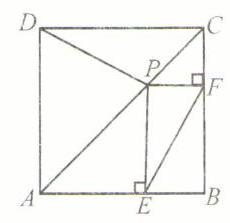
\includegraphics[width=0.2\textwidth]{bodyxb/src/bo_d20aucref24c73anc48g_25_1206_136_230_223_0.jpg}
\end{center}


(图 6)

$\because A,P,C$ 三点共线, $\therefore \vv{AP} = t\left( {\vv{a} + \vv{b}}\right)$ .

$\therefore \vv{DP} = \vv{AP} - \vv{AD} = t\left( {\vv{a} + \vv{b}}\right)  - \vv{b} = t\vv{a} + \left( {t - 1}\right) \vv{b}$ .

又 $\because \vv{AE} = {ta},\therefore \vv{PF} = \left( {1 - t}\right) a,\vv{EP} = {tb}$ .

$\therefore \vv{EF} = \vv{EP} + \vv{PF} = {tb} + \left( {1 - t}\right) \vv{a}$ .

$\therefore \vv{DP} \cdot  \vv{EF} = \left\lbrack  {{ta} + \left( {t - 1}\right) \vv{b}}\right\rbrack   \cdot  \left\lbrack  {t\vv{b} + \left( {1 - t}\right) \vv{a}}\right\rbrack   = 0,\therefore {PD} \bot  {EF}.$

例 2 如图 7,在 $\bigtriangleup {ABC}$ 中, $M$ 是 ${BC}$ 的中点,点 $N$ 在边 ${AC}$ 上,且 ${AN} = {2NC},{AM}$ 与 ${BN}$ 交于点 $P$ ,求 ${AP} : {PM}$ 的值.

解 设 $\vv{BM} = a,\vv{CN} = b$ ,则 $\vv{AM} = \vv{AC} + \vv{CM} =  - a - {3b},\vv{BN} = {2a} + b$ .

$\because A,P,M$ 三点共线, $B,P,N$ 三点共线,

\begin{center}
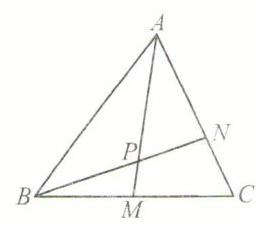
\includegraphics[width=0.2\textwidth]{bodyxb/src/bo_d20aucref24c73anc48g_25_1175_646_261_228_0.jpg}
\end{center}


(图 7)

$\therefore$ 存在实数 $\lambda ,\mu$ ,使 $\vv{AP} = \lambda \vv{AM} =  - {\lambda a} - {3\lambda b},\vv{BP} = \mu \vv{BN} = {2\mu a} + {\mu b}$ .

$\therefore \vv{BA} = \vv{BP} - \vv{AP} = \left( {\lambda  + {2\mu }}\right) \vv{a} + \left( {{3\lambda } + \mu }\right) \vv{b}$ .

又 $\because \vv{BA} = \vv{BC} + \vv{CA} = 2\vv{a} + 3\vv{b}$ ,

$\therefore$ 由平面向量基本定理,得 $\left\{  {\begin{array}{l} \lambda  + {2\mu } = 2, \\  {3\lambda } + \mu  = 3 \end{array} \Rightarrow  \left\{  \begin{array}{l} \lambda  = \dfrac{4}{5}, \\  \mu  = \dfrac{3}{5}, \end{array}\right. }\right.$

从而 $\vv{AP} = \dfrac{4}{5}\vv{AM}.\therefore {AP} : {PM} = 4 : 1$ . 2. 在物理中的应用. 物理中的有关力、速度、位移等问题,可运用向量方法解答. 例 3 已知向量 ${e}_{1} = \left( {1,0}\right) ,{e}_{2} = \left( {0,1}\right)$ . 现有动点 $P$ 从点 ${P}_{0}\left( {-1,2}\right)$ 出发,沿着与向量 ${e}_{1} +$  ${\vv{e}}_{2}$ 相同的方向做匀速直线运动,速度大小为 $\left| {{\vv{e}}_{1} + {\vv{e}}_{2}}\right|$ ; 另一点 $Q$ 从点 ${Q}_{0}\left( {-2, - 1}\right)$ 出发,沿着与向量 $3{\vv{e}}_{1} + 2{\vv{e}}_{2}$ 相同的方向做匀速直线运动,速度大小为 $\left| {3{\vv{e}}_{1} + 2{\vv{e}}_{2}}\right|$ . 设点 $P,Q$ 在时刻 $t = 0$ 时分别在点 ${P}_{0},{Q}_{0}$ 处,当运动多长时间时, $\vv{PQ} \bot  \vv{{P}_{0}{Q}_{0}}$ ?

解 由题意,设点 $P\left( {{x}_{1},{y}_{1}}\right) ,Q\left( {{x}_{2},{y}_{2}}\right)$ ,则

$\left( {{x}_{1},{y}_{1}}\right)  = \left( {-1,2}\right)  + \left( {1,1}\right) t = \left( {-1 + t,2 + t}\right) ,$

$\left( {{x}_{2},{y}_{2}}\right)  = \left( {-2, - 1}\right)  + \left( {3,2}\right) t = \left( {-2 + {3t}, - 1 + {2t}}\right) .$

$\therefore \vv{PQ} = \left( {-1 + {2t}, - 3 + t}\right) ,\vv{{P}_{0}{Q}_{0}} = \left( {-1, - 3}\right)$ .

$\because \vv{PQ} \bot  \vv{{P}_{0}{Q}_{0}},\therefore \vv{PQ} \cdot  \vv{{P}_{0}{Q}_{0}} = 0,\therefore \left( {-1}\right) \left( {-1 + {2t}}\right)  + \left( {-3}\right) \left( {-3 + t}\right)  = 0$ ,

$\therefore t = 2$ . 因此,运动 $2\mathrm{s}$ 时, $\vv{PQ}\bot \vv{{P}_{0}{Q}_{0}}$ .

例 4 如图 8,在 $O$ 处用水平力 ${\vv{F}}_{2}$ 缓慢拉起重为 $\vv{G}$ 的物体,绳子与铅垂线方向的夹角为 $\theta$ ,绳子所受到的拉力为 ${\vv{F}}_{1}$ .

(1)分析 $\left| {\vv{F}}_{1}\right| ,\left| {\vv{F}}_{2}\right|$ 随 $\theta$ 的变化而变化的情况；

(2)当 $\left| {\vv{F}}_{1}\right|  \leq  2\left| \vv{G}\right|$ 时,求 $\theta$ 的取值范围.

解 由题意可知, ${\vv{F}}_{1},{\vv{F}}_{2},\vv{G}$ 三者的关系如图 9 所示.

(1)以力 ${\vv{F}}_{1},{\vv{F}}_{2}$ 所在的线段 ${OA},{OB}$ 为邻边作 $▱{OACB}$ ,则 $\left| {\vv{F}}_{1}\right|  = \dfrac{\left| \vv{G}\right| }{\cos \theta }$ , $\left| {\vv{F}}_{2}\right|  = \left| \vv{G}\right| \tan \theta ,\theta  \in  \left( {0,\dfrac{\pi }{2}}\right)$ . 因此, $\left| {\vv{F}}_{1}\right| ,\left| {\vv{F}}_{2}\right|$ 随 $\theta$ 的变大而变大.

\begin{center}
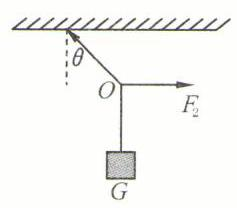
\includegraphics[width=0.2\textwidth]{bodyxb/src/bo_d20aucref24c73anc48g_26_496_324_237_208_0.jpg}
\end{center}


(图 8)

\begin{center}
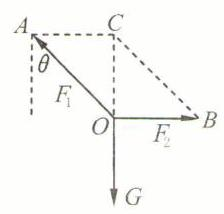
\includegraphics[width=0.2\textwidth]{bodyxb/src/bo_d20aucref24c73anc48g_26_965_318_224_214_0.jpg}
\end{center}


(图 9)

(2)当 $\left| {\vv{F}}_{1}\right|  \leq  2\left| \vv{G}\right|$ ,即 $\dfrac{\left| \vv{G}\right| }{\cos \theta } \leq  2\left| \vv{G}\right|$ 时, $\cos \theta  \geq  \dfrac{1}{2}$ .

$\because \theta  \in  \left( {0,\dfrac{\pi }{2}}\right) ,\therefore \theta  \in  \left( {0,\dfrac{\pi }{3}}\right\rbrack  .$

3. 在三角函数中的应用.

把三角函数问题转化为向量问题, 利用向量的运算加以解决.

例 5 在 $\bigtriangleup {ABC}$ 中, ${AB} = \dfrac{4}{3}\sqrt{6},\cos B = \dfrac{\sqrt{6}}{6}$ ,边 ${AC}$ 上的中线 ${BD} = \sqrt{5}$ ,求 $\sin A$ 的值.

解 如图 10,以 $B$ 为坐标原点, $\vv{BC}$ 为 $x$ 轴正方向建立平面直角坐标系. 不妨设点 $A$ 位于第一象限.

由 $\sin B = \dfrac{\sqrt{30}}{6}$ ,得 $\vv{BA} = \left( {\dfrac{4\sqrt{6}}{3}\cos B,\dfrac{4\sqrt{6}}{3}\sin B}\right)  = \left( {\dfrac{4}{3},\dfrac{4\sqrt{5}}{3}}\right)$ .

设 $\vv{BC} = \left( {x,0}\right)$ ,则 $\vv{BD} = \left( {\dfrac{4 + {3x}}{6},\dfrac{2\sqrt{5}}{3}}\right)$ .

\begin{center}
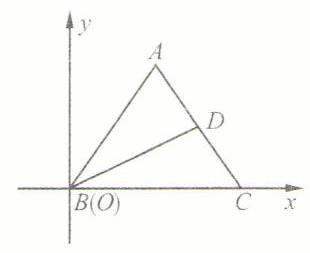
\includegraphics[width=0.2\textwidth]{bodyxb/src/bo_d20aucref24c73anc48g_26_1208_1251_310_253_0.jpg}
\end{center}


(图 10)

由条件,得 $\left| \vv{BD}\right|  = \sqrt{{\left( \dfrac{4 + {3x}}{6}\right) }^{2} + {\left( \dfrac{2\sqrt{5}}{3}\right) }^{2}} = \sqrt{5}$ .

从而 $x = 2$ ,或 $x =  - \dfrac{14}{3}$ (不合题意,舍去).

故 $\vv{CA} = \left( {-\dfrac{2}{3},\dfrac{4\sqrt{5}}{3}}\right)$ ,

于是 $\cos A = \dfrac{\vv{BA} \cdot  \vv{CA}}{\left| \vv{BA}\right| \left| \vv{CA}\right| } = \dfrac{-\dfrac{8}{9} + \dfrac{80}{9}}{\sqrt{\dfrac{16}{9} + \dfrac{80}{9}}\sqrt{\dfrac{4}{9} + \dfrac{80}{9}}} = \dfrac{3\sqrt{14}}{14}$ ,

$\therefore \sin A = \sqrt{1 - {\cos }^{2}A} = \dfrac{\sqrt{70}}{14}$ .

4. 两点距离公式的应用.

两点 $P\left( {{x}_{1},{y}_{1}}\right) ,Q\left( {{x}_{2},{y}_{2}}\right)$ 的距离: $\left| {PQ}\right|  = \sqrt{{\left( {x}_{2} - {x}_{1}\right) }^{2} + {\left( {y}_{2} - {y}_{1}\right) }^{2}}$ .

特别地. 点 $P\left( {x,y}\right)$ 和原点 $O\left( {0,0}\right)$ 的距离是 $\left| {PO}\right|  = \sqrt{{x}^{2} + {y}^{2}}$ .

例 6 如图 11,在 $y$ 轴上求一点 $P$ ,使得点 $P$ 和点 $A\left( {-2,5}\right) ,B\left( {1, - 4}\right)$ 等距离.

解 设点 $P$ 的坐标为(0, b),则 $\sqrt{4 + {\left( b - 5\right) }^{2}} = \sqrt{1 + {\left( b + 4\right) }^{2}}$ ,

\begin{center}
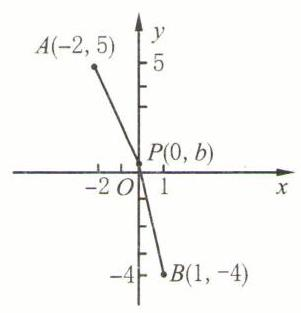
\includegraphics[width=0.2\textwidth]{bodyxb/src/bo_d20aucref24c73anc48g_27_1138_195_301_313_0.jpg}
\end{center}


(图 11)

平方得 ${b}^{2} - {10b} + {29} = {b}^{2} + {8b} + {17}$ ,即 ${18b} = {12},\therefore b = \dfrac{2}{3}$ .

故点 $P$ 的坐标为 $P\left( {0,\dfrac{2}{3}}\right)$ .

例 7 已知 $f\left( x\right)  = \sqrt{1 + {x}^{2}}$ ,求证: $\left| {f\left( a\right)  - f\left( b\right) }\right|  \leq  \left| {a - b}\right|$ .

证明 如图 12,设点 $A,B$ 的坐标依次为 $\left( {1,a}\right) ,\left( {1,b}\right)$ ,则

$f\left( a\right)  = \sqrt{1 + {a}^{2}} = \left| {AO}\right| ,f\left( b\right)  = \sqrt{1 + {b}^{2}} = \left| {BO}\right| ,\left| {a - b}\right|  = \left| {AB}\right|$ .

当 $a \neq  b$ 时,在 $\bigtriangleup {AOB}$ 中,由 $\left| {AO}\right|  - \left| {BO}\right| \left|  < \right| {AB} \mid$ ,即得 $\left| {f\left( a\right)  - f\left( b\right) }\right|  < \left| {a - b}\right| .$

\begin{center}
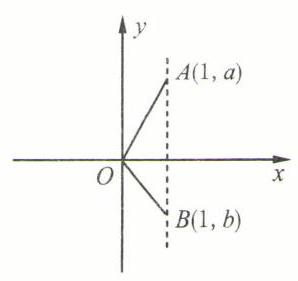
\includegraphics[width=0.2\textwidth]{bodyxb/src/bo_d20aucref24c73anc48g_27_1141_648_298_281_0.jpg}
\end{center}


(图 12)

当 $a = b$ 时, $\left| {OA}\right|  = \left| {OB}\right| ,\left| {a - b}\right|  = 0$ ,

故有 $\left| {f\left( a\right)  - f\left( b\right) }\right|  = \left| {a - b}\right|$ .

综上所述,便得 $\left| {f\left( a\right)  - f\left( b\right) }\right|  \leq  \left| {a - b}\right|$ .

5. 定比分点的应用.

在应用定比分点时,应该注意两点:

(1)公式的“逆用”.

例 8 如图 13,已知两点 $A\left( {4,1}\right)$ 和 $B\left( {-1,3}\right)$ ,求线段 ${AB}$ 和 $y$ 轴交点 $M$ 的坐标.

解 设点 $M$ 的坐标为 $\left( {0,{y}_{0}}\right)$ ,且 $\dfrac{AM}{MB} = \lambda$ ,则由定比分点公式得 $0 = \dfrac{4 + \lambda \left( {-1}\right) }{1 + \lambda },\therefore \lambda  = 4,$

\begin{center}
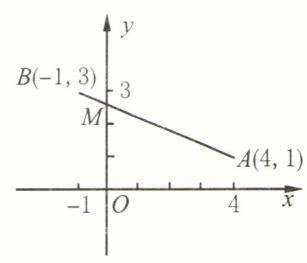
\includegraphics[width=0.2\textwidth]{bodyxb/src/bo_d20aucref24c73anc48g_27_1128_1168_307_263_0.jpg}
\end{center}


(图 13)

于是 ${y}_{0} = \dfrac{1 + 4 \times  3}{1 + 4} = \dfrac{13}{5}$ ,即点 $M$ 的坐标是 $M\left( {0,\dfrac{13}{5}}\right)$ .

(2)注意利用平面几何知识.

例 9 如图 14,已知 $A\left( {5, - 1}\right) ,B\left( {-1,7}\right) ,C\left( {1,2}\right)$ ,求 $\bigtriangleup {ABC}$ 中 $\angle A$ 的平分线 ${AD}$ 的长.

解 ∵ $\left| {AB}\right|  = \sqrt{{\left( 1 + 5\right) }^{2} + {\left( 7 + 1\right) }^{2}} = {10}$ ,

\begin{center}
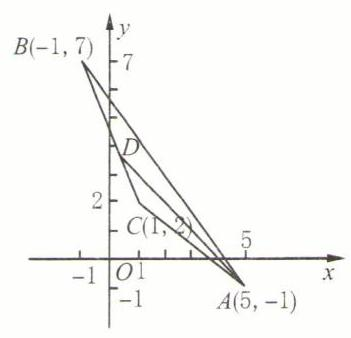
\includegraphics[width=0.3\textwidth]{bodyxb/src/bo_d20aucref24c73anc48g_27_1085_1579_351_338_0.jpg}
\end{center}


(图 14)

$\left| {AC}\right|  = \sqrt{{\left( 5 - 1\right) }^{2} + {\left( 2 + 1\right) }^{2}} = 5.$

则由 $\lambda  = \dfrac{\left| BD\right| }{\left| CD\right| } = \dfrac{\left| AB\right| }{\left| AC\right| } = 2$ ,

设点 $D\left( {{x}_{0},{y}_{0}}\right)$ ,则 ${x}_{0} = \dfrac{-1 + 2 \times  1}{1 + 2} = \dfrac{1}{3},{y}_{0} = \dfrac{7 + 2 \times  2}{1 + 2} = \dfrac{11}{3}$ ,

即 $D\left( {\dfrac{1}{3},\dfrac{11}{3}}\right)$ ,于是 $\left| {AD}\right|  = \sqrt{{\left( 5 - \dfrac{1}{3}\right) }^{2} + {\left( -1 - \dfrac{11}{3}\right) }^{2}} = \dfrac{14}{3}\sqrt{2}$ .

注意 本例运用了三角形角平分线的性质: 若 ${AD}$ 是 $\bigtriangleup {ABC}$ 的内角平分线,则 $\left| {AB}\right|$ : $\left| {AC}\right|  = \left| {BD}\right|$ : $\left| {CD}\right|$ (你会证明吗?). 在学习解析几何时,要尽可能地发掘出所给图形的几何性质, 简化解题.

\section*{(A)}

187. 已知点 $A\left( {1,2}\right) ,B\left( {2,3}\right) ,C\left( {-2,5}\right)$ ,那么 $\bigtriangleup  {ABC}$ 的形状是(   )

(A) 锐角三角形. (B) 等边三角形. (C) 钝角三角形. (D) 直角三角形.

188. 已知四边形 ${ABCD}$ 的三个顶点 $A\left( {0,2}\right) ,B\left( {-1, - 2}\right) ,C\left( {3,1}\right)$ ,且 $\vv{BC} = 2\vv{AD}$ ,那么顶点 $D$ 的坐标为 (   )

(A) $\left( {2,\dfrac{7}{2}}\right)$ . (B) $\left( {2, - \dfrac{1}{2}}\right)$ . (C)(3,2). (D)(1,3).

189. 已知向量 $\vv{AB} = \left( {2,1}\right) ,\vv{AC} = \left( {3,k}\right)$ . 若 $\bigtriangleup {ABC}$ 是直角三角形,则实数 $k$ 的可能值的个数是(   )

(A) 1 . (B) 2 . (C) 3. (D) 4.

190. 若某人骑自行车的速度为 ${v}_{1}$ ,风速为 ${v}_{2}$ ,则此人逆风行驶时的速度大小为(   )

(A) ${v}_{1} - {v}_{2}$ . (B) ${v}_{1} + {v}_{2}$ . (C) $\left| {\vv{v}}_{1}\right|  - \left| {\vv{v}}_{2}\right|$ . (D) $\dfrac{\left| {\vv{v}}_{1}\right| }{\left| {\vv{v}}_{2}\right| }$ .

191. 若两人提重为 $\left| \vv{G}\right|$ 的一桶水,夹角为 $\theta$ ,用力为 $\vv{F}$ ,则 (   )

(A) $\left| \vv{F}\right|  = \dfrac{\left| \vv{G}\right| }{2\cos \theta }$ . (B) $\left| \vv{F}\right|  = \dfrac{\left| \vv{G}\right| }{2\sin \theta }$ .

(C) $\left| \vv{F}\right|  = \dfrac{\left| \vv{G}\right| }{2\cos \dfrac{\theta }{2}}$ . (D) $\left| \vv{F}\right|  = \dfrac{\left| \vv{G}\right| }{2\sin \dfrac{\theta }{2}}$ .

192. 已知 $▱{ABCD}$ 的两个顶点 $A\left( {-\dfrac{9}{2}, - 7}\right) ,B\left( {2,6}\right)$ ,对角线的交点为 $M\left( {3,\dfrac{3}{2}}\right)$ ,则另两个顶点 $C,D$ 的坐标分别为\blkda{}.

193. 在 $\bigtriangleup {ABC}$ 中,点 $A\left( {0,7}\right) ,B\left( {-4,5}\right)$ ,重心 $G\left( {0,\dfrac{1}{3}}\right)$ ,则边 ${AB}$ 上的中线 ${CD}$ 的长为\blkda{}.

194. 某人以时速 $v\mathrm{{km}}$ 向东行走,此时正刮着时速 $v\mathrm{{km}}$ 的南风,那么此人感到的风向为\blkda{},风速为\blkda{} km/h.

195. 用两条夹角为 ${60}^{ \circ  }$ 的绳索拉船,每条绳索上的拉力是 ${12}\mathrm{N}$ ,则合力为\blkda{}(精确到 ${0.1}\mathrm{N}$ ).

196. 求证: 对边平方和相等的四边形的对角线互相垂直.

197. 求证: 平行四边形的对角线的平方和等于相邻两边的平方和的两倍.

198. 试证明 $\bigtriangleup {ABC}$ 的三条高线交于一点.

\begin{center}
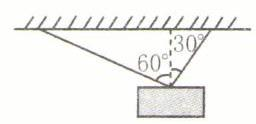
\includegraphics[width=0.2\textwidth]{bodyxb/src/bo_d20aucref24c73anc48g_28_1232_1959_256_124_0.jpg}
\end{center}


(第 199 题)

199. 如图,在重 ${400}\mathrm{N}$ 的物体上,系两根绳子,这两根绳子在铅垂线的两侧,与铅垂线的夹角分别是 ${30}^{ \circ  },{60}^{ \circ  }$ ,求平衡时两根绳子拉力的大小.

200. 如图,一条两岸为平行直线的小河,河宽 $L = {60}\mathrm{m}$ ,水流速度为 $5\mathrm{m}/\mathrm{s}$ . 一小船欲从码头 $A$ 处渡河过去,码头 $A$ 的下游 ${80}\mathrm{m}$ 处的河床陡然降低形成瀑布 $B$ . 要保证小船不掉下瀑布,小船相对水的划行速度至少应多大? 此时船的划行方向如何?

\begin{center}
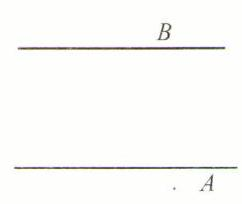
\includegraphics[width=0.2\textwidth]{bodyxb/src/bo_d20aucref24c73anc48g_29_1194_120_242_204_0.jpg}
\end{center}


(第 200 题)

201. 已知两点 $A\left( {\cos \alpha ,\sin \alpha }\right)$ 和 $B\left( {\cos {2\alpha },\sin {2\alpha }}\right)$ ,则 ${AB}$ 的长为(   )

(A) $2\sin \dfrac{\alpha }{2}$ . (B) $2\left| {\sin \dfrac{\alpha }{2}}\right|$ . (C) $2\cos \dfrac{\alpha }{2}$ . (D) $2\left| {\cos \dfrac{\alpha }{2}}\right|$ .

202. 若 $x$ 轴上的点 $M$ 到原点及点(5, - 3)的距离相等,则点 $M$ 的坐标是(   )

(A)(-2,0). (B)(1,0). (C)(1.5,0). (D)(3.4,0).

203. 已知两点 $P\left( {\cos \alpha ,\sin \alpha }\right) ,Q\left( {\cos \beta ,\sin \beta }\right)$ ,则 $\left| {PQ}\right|$ 的最大值是 (   )

(A) $\sqrt{2}$ . (B) 2 . (C) 4. (D) 不存在.

204. 若点 $P$ 在直线 ${P}_{1}{P}_{2}$ 上,且 $\vv{{P}_{1}P} = \lambda \vv{P{P}_{2}}$ ,则下列结论中,正确的是 (   )

(A) $\lambda$ 恒大于零.

(B) 若 $\lambda  < 0$ 且 $\lambda  \neq   - 1$ ,则点 $P$ 必在 ${P}_{1}{P}_{2}$ 的延长线上.

(C) 若 $\lambda  =  - 1$ ,则点 $P$ 与 ${P}_{2}$ 重合.

(D) 若 $\lambda  = 0$ ,则点 $P$ 与 ${P}_{1}$ 重合.

205. 若点 $P$ 在直线 ${AB}$ 上,且 $\vv{AP} = \dfrac{1}{3}\vv{PB}$ . 设 $\vv{AB} = t\vv{BP}$ ,则 $t$ 的值为 (   )

(A) $\dfrac{4}{3}$ . (B) $\dfrac{3}{4}$ . (C) $- \dfrac{4}{3}$ . (D) $- \dfrac{3}{4}$ .

206. 已知两点 $A\left( {m, - n}\right) ,B\left( {-m,n}\right)$ ,又 $\vv{AC} =  - 2\vv{CB}$ ,那么点 $C$ 的坐标为 (   )

(A)(-3m,3n). (B)(m, n).

(C)(3m,3n). (D)(-m, n).

207. 已知两点 $P\left( {-1, - 6}\right)$ 和 $Q\left( {3,0}\right)$ ,延长 ${QP}$ 到点 $A$ ,使 $\left| {AP}\right|  = \dfrac{1}{3}\left| {PQ}\right|$ ,那么点 $A$ 的坐标为(   )

(A) $\left( {-\dfrac{7}{3}, - 8}\right)$ . (B) $\left( {0,\dfrac{9}{2}}\right)$ . (C) $\left( {\dfrac{2}{3}, - 2}\right)$ . (D) $\left( {-\dfrac{2}{3},2}\right)$ .

208. 已知点 $P\left( {4, - 9}\right)$ 与点 $Q\left( {-2,3}\right)$ ,设 $y$ 轴与直线 ${PQ}$ 的交点为 $M$ ,且 $\vv{PM} = \lambda \vv{QM}$ ,则 $\lambda$ 的值为(   )

(A) $\dfrac{1}{3}$ . (B) $\dfrac{1}{2}$ . (C) 2 . (D) 3.

209. 直线上有 $A,B,C$ 三点,如果 $\vv{AB} =  - \dfrac{1}{2}\vv{BC}$ ,则(   )

(A) $B$ 是线段 ${AC}$ 的中点. (B) $A$ 是线段 ${BC}$ 的中点.

(C) $C$ 是线段 ${AB}$ 的中点. (D) $B$ 是线段 ${AC}$ 的三等分点.

210. 在 $\bigtriangleup {ABC}$ 中,已知 $A\left( {2,3}\right) ,B\left( {8, - 4}\right)$ ,重心 $G\left( {2, - 1}\right)$ ,则点 $C$ 的坐标为(   )

(A)(-4,2). (B)(-4, - 2). (C)(4, - 2). (D)(4,2).

211. (1)已知两点 $A\left( {1,5}\right)$ 和 $B\left( {x,2}\right)$ 的距离为 5,则点 $B$ 的横坐标是\blkda{}；

(2)若点 $M$ 在 $y$ 轴上,且与点 $\left( {-4, - 1}\right) ,\left( {2,3}\right)$ 等距离,则点 $M$ 的坐标是\blkda{}；

(3)若点 $Q$ 与点 ${P}_{1}\left( {0,1}\right)$ , ${P}_{2}\left( {7,2}\right)$ 及 $x$ 轴等距离,则点 $Q$ 的坐标是\blkda{}.

212. (1) 若点 $P\left( {x,1}\right)$ 在 $A\left( {2, - 4}\right) ,B\left( {5,{11}}\right)$ 这两点的连线上,则 $x =$ \blkda{}；

(2)连接 $A\left( {4,1}\right)$ 和 $B\left( {-2,4}\right)$ 两点的直线,和 $x$ 轴交点的坐标是\blkda{},和 $y$ 轴交点的坐标是\blkda{}；

(3)已知点 ${P}_{1},{P}_{2},{P}_{3}$ 共线,且 $\vv{{P}_{1}{P}_{3}} =  - \dfrac{2}{3}\vv{{P}_{3}{P}_{2}}$ ,设 $\vv{{P}_{1}{P}_{2}} = t\vv{{P}_{3}{P}_{1}}$ ,则 $t =$ \blkda{}；

(4)已知 $A\left( {4,2}\right) ,B\left( {-6, - 4}\right) ,C\left( {x, - 2\dfrac{4}{5}}\right)$ 三点共线,且 $\vv{AC} = \lambda \vv{CB}$ ,则 $\lambda  =$ \blkda{}, $x =$ \blkda{};

(5)已知点 $A\left( {3, - 4}\right)$ 与 $B\left( {-1,2}\right)$ ,点 $P$ 在直线 ${AB}$ 上,且 $\left| {PA}\right|  = 2\left| {PB}\right|$ ,则点 $P$ 的坐标是\blkda{}；

(6) 已知 $\vv{{P}_{1}P} = \lambda \vv{P{P}_{2}}$ .

①若 $P$ 在线段 ${P}_{1}{P}_{2}$ 内,则 $\lambda  \in$ \blkda{},

②若 $P$ 在线段 ${P}_{1}{P}_{2}$ 的延长线上,则 $\lambda  \in$ \blkda{},

③若 $P$ 在线段 ${P}_{2}{P}_{1}$ 的延长线上,则 $\lambda  \in$ \blkda{}.

213. (1) 已知同一直线上三点 $A\left( {x,5}\right) ,B\left( {-2,y}\right) ,C\left( {1,1}\right)$ 满足 $\left| {BC}\right|  = 2\left| {AC}\right|$ ,求 $x$ , $y$ 的值;

(2)在 $\bigtriangleup {ABC}$ 中,已知顶点 $A$ 的坐标为 $\left( {3,1}\right) ,{AB}$ 的中点为 $D\left( {2,4}\right) ,\bigtriangleup {ABC}$ 的重心为 $G\left( {3,4}\right)$ ,求顶点 $B,C$ 的坐标.

\begin{center}
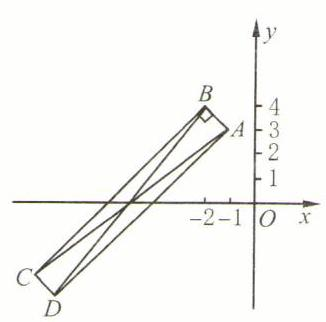
\includegraphics[width=0.2\textwidth]{bodyxb/src/bo_d20aucref24c73anc48g_30_1186_1124_326_322_0.jpg}
\end{center}


[第 214(2)题]

214. (1) 在等腰直角三角形 ${ABC}$ 中,已知 $\angle {ABC} = {90}^{ \circ  }$ ,顶点 $A(1$ , $0),B\left( {3,1}\right)$ ,求顶点 $C$ 的坐标;

(2)在矩形 ${ABCD}$ 中,已知顶点 $A\left( {-1,3}\right) ,B\left( {-2,4}\right)$ ,其对角线的交点在 $x$ 轴上 (如图),求顶点 $C,D$ 的坐标.

\section*{(B)}

215. 已知 $\bigtriangleup  {ABC}$ 的顶点为 $A\left( {0,8}\right) ,B\left( {-4,0}\right) ,C\left( {5, - 3}\right)$ . 若点 $D$ 在边 ${BC}$ 上,且 $\bigtriangleup  {ABD}$ 的面积是 $\bigtriangleup {ABC}$ 的 $\dfrac{1}{3}$ ,则点 $D$ 的坐标为 (   )

(A)(3, - 1). (B)(-1, - 1). (C) $\left( {\dfrac{1}{3},1}\right)$ . (D) $\left( {-\dfrac{1}{3}, - 1}\right)$ .

216. 如图,正方形 ${ABCD}$ 的边长为 $2,M$ 是 ${BC}$ 的中点,将正方形 ${ABCD}$ 折起,使点 $A$ 与点 $M$ 重合. 设折痕为 ${EF}$ ,则 ${AE}$ 的长为(   )

\begin{center}
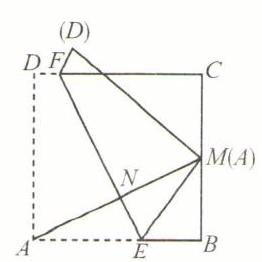
\includegraphics[width=0.2\textwidth]{bodyxb/src/bo_d20aucref24c73anc48g_30_1246_1883_262_262_0.jpg}
\end{center}


(第 216 题)

(A) 1 . (B) $\dfrac{3}{2}$ .

(C) $\dfrac{5}{4}$ . (D) $\dfrac{4}{3}$ .

217. 已知 $G$ 是 $\bigtriangleup {ABC}$ 的重心,过点 $G$ 的任意一条直线交 ${AB}$ 于点 $Q$ ,交 ${AC}$ 于点 $P$ . 若 ${AQ} =$  $\dfrac{1}{m}{AB},{AP} = \dfrac{1}{n}{AC}$ ,则 $m + n$ 等于 (   )

(A) 1 . (B) 2 . (C) 3. (D) 4.

218. 力 $\vv{F}$ 的两个分力的方向与力 $\vv{F}$ 成相同的角度,称两个分力的方向关于力 $\vv{F}$ 是对称的. 当两个对称的分力的夹角增大时,两个分力的大小 (   )

(A) 先小后大. (B) 先大后小. (C) 越来越大. (D) 越来越小.

219. 一只船要横渡一条 ${30}\mathrm{m}$ 宽的河,它在静水中的速度为 $3\mathrm{m}/\mathrm{s}$ . 水流的速度为 $4\mathrm{m}/\mathrm{s}$ ,下列说法正确的是(   )

(A)这只船可能垂直于河岸到达对岸. (B) 这只船对地的速度是 $5\mathrm{m}/\mathrm{s}$ .

(C) 过河时间可能是 $6\mathrm{s}$ . (D) 过河时间可能是 ${12}\mathrm{s}$ .

220. 已知两个力 ${\vv{F}}_{1},{\vv{F}}_{2}$ 的夹角是 ${90}^{ \circ  }$ ,它们的合力 $\vv{F}$ 的大小为 ${10}\mathrm{N}$ . 若 ${\vv{F}}_{1}$ 的大小为 $6\mathrm{N}$ ,则 ${\vv{F}}_{2} =$ \blkda{}N.

221. 若三个力 ${\vv{F}}_{1} = \left( {3,4}\right) ,{\vv{F}}_{2} = \left( {2, - 5}\right) ,{\vv{F}}_{3} = \left( {x,y}\right)$ ,且 ${\vv{F}}_{1} + {\vv{F}}_{2} + {\vv{F}}_{3} = \vv{0}$ ,则 ${\vv{F}}_{3}$ 的坐标为\blkda{}.

222. 若质点 $P$ 由点 $A\left( {2,1}\right)$ 移动到点 $B\left( {5,5}\right)$ (单位: $\mathrm{m}$ ),则位移 $\vv{AB} =$ \blkda{},恒力 $\vv{F} =$  $4\vv{i} + 3\vv{j}$ (单位为 $\mathrm{N}$ )对质点 $P$ 所做的功 $W =$ \blkda{} $\mathrm{J}$ .

223. 若矩形 ${ABCD}$ 的三个顶点为 $A\left( {2,1}\right) ,B\left( {3,2}\right) ,D\left( {-1,4}\right)$ ,则顶点 $C$ 的坐标为\blkda{}.

224. 若 $\bigtriangleup {ABC}$ 的三个顶点为 $A\left( {4,1}\right) ,B\left( {7,5}\right) ,C\left( {-4,7}\right) ,{AF}$ 是 $\angle {BAC}$ 的平分线,则 ${AF}$ 的长为\blkda{}.

225. 已知正三角形 ${ABC}$ 的边长为 $a,P$ 是平面上任意一点. 当 ${\left| \vv{PA}\right| }^{2} + {\left| \vv{PB}\right| }^{2} + {\left| \vv{PC}\right| }^{2}$ 最小时,点 $P$ 的位置在\blkda{},此时, ${\left| \vv{PA}\right| }^{2} + {\left| \vv{PB}\right| }^{2} + {\left| \vv{PC}\right| }^{2} =$ \blkda{}.

226. 如图,在 ▱ ${ABCD}$ 的对角线 ${BD}$ 所在的直线上,取两点 $E$ , $F$ ,使 ${BE}$  $= {DF}$ . 用向量方法证明: 四边形 ${AECF}$ 也是平行四边形.

\begin{center}
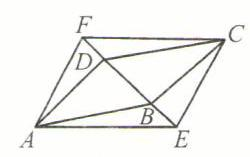
\includegraphics[width=0.2\textwidth]{bodyxb/src/bo_d20aucref24c73anc48g_31_1176_1362_250_157_0.jpg}
\end{center}


(第 226 题)

227. 在平面上有两个三角形, $\bigtriangleup {A}_{1}{B}_{1}{C}_{1}$ 和 $\bigtriangleup {A}_{2}{B}_{2}{C}_{2}$ ,它们的重心分别为 ${G}_{1},{G}_{2}$ . 求证: $\left| \vv{{G}_{1}{G}_{2}}\right|  \leq  \left| \vv{{A}_{1}{A}_{2}}\right|  + \left| \vv{{B}_{1}{B}_{2}}\right|  + \left| \vv{{C}_{1}{C}_{2}}\right|$ .

228. 求证: 从任意四个不同的实数 ${a}_{1},{a}_{2},{a}_{3},{a}_{4}$ 中,一定存在两个不同的实数 ${a}_{i},{a}_{j}\left( {i < j}\right)$ ,使得 $1 + {a}_{i}{a}_{j} > \dfrac{1}{2}\sqrt{\left( {1 + {a}_{i}^{2}}\right) \left( {1 + {a}_{j}^{2}}\right) }$ .

229. 以 $E\left( {3, - 5}\right) ,F\left( {2,2}\right) ,G\left( {-5,1}\right)$ 为顶点的三角形的外心坐标是 (   )

(A)(0,0). (B)(-1,0). (C)(-1, - 2). (D)(2, - 1).

230. 已知一个平行四边形的三个顶点是 $\left( {4,2}\right) ,\left( {5,7}\right) ,\left( {-3,4}\right)$ ,则第四个顶点不可能是(   )

(A)(12,5). (B)(-2,9). (C)(-4, - 1). (D)(3,7).

231. 已知两点 $A\left( {{x}_{1},{y}_{1}}\right) ,B\left( {{x}_{2},{y}_{2}}\right) ,P$ 是直线 ${AB}$ 上一点,且 $\vv{AP} = \lambda \vv{AB}$ ,则点 $P$ 的坐标为(   )

(A) $\left( {\dfrac{{x}_{1} + \lambda {x}_{2}}{1 + \lambda },\dfrac{{y}_{1} + \lambda {y}_{2}}{1 + \lambda }}\right)$ . (B) $\left( {\dfrac{{x}_{2} + \lambda {x}_{1}}{1 + \lambda },\dfrac{{y}_{2} + \lambda {y}_{1}}{1 + \lambda }}\right)$ .

(C) $\left( {\lambda {x}_{1} + \left( {1 - \lambda }\right) {x}_{2},\lambda {y}_{1} + \left( {1 - \lambda }\right) {y}_{2}}\right)$ . (D) $\left( {\lambda {x}_{2} + \left( {1 - \lambda }\right) {x}_{1},\lambda {y}_{2} + \left( {1 - \lambda }\right) {y}_{1}}\right)$ .

232. 连接直角三角形的直角顶点和斜边的两个三等分点,所得两条线段的长分别是 $\sin \alpha$ 和 $\cos \alpha \left( {0 < \alpha  < \dfrac{\pi }{2}}\right)$ ,则斜边的长为 (   )

(A) $\dfrac{4}{3}$ . (B) $\dfrac{3}{\sqrt{5}}$ . (C) $\dfrac{2}{\sqrt{5}}$ . (D) $\sqrt{5}$ .

233. (1) 已知点 $A\left( {3,4}\right) ,B\left( {1,2}\right)$ ,直线 ${AB}$ 上的点 $P$ 满足 $\left| \dfrac{AP}{AB}\right|  = \dfrac{1}{3}$ ,则点 $P$ 的坐标为\blkda{}；

(2)已知 $A\left( {-1,2}\right) ,B\left( {1,1}\right) ,C\left( {-1, - 1}\right)$ 是 $\bigtriangleup  {ABC}$ 的三个顶点,延长 ${AB}$ 至 $P$ ,使 $B$ 为 ${AP}$ 的中点,延长 ${CP}$ 至 $Q$ ,使 $P$ 为 ${CQ}$ 的中点,则点 $Q$ 的坐标为\blkda{}；

(3)已知 $\bigtriangleup  {ABC}$ 的三边的中点分别为 $\left( {2, - 1}\right) ,\left( {-1,4}\right) ,\left( {-2,2}\right)$ ,则 $\bigtriangleup  {ABC}$ 的重心坐标为\blkda{}.

234. (1) 已知 $\bigtriangleup {ABC}$ 的三个顶点是 $A\left( {4,1}\right) ,B\left( {7,5}\right)$ 和 $C\left( {-4,7}\right)$ ,求此三角形的内角 $\angle {BAC}$ 的平分线的长;

(2)已知 $\bigtriangleup  {ABC}$ 的三边长 ${BC} = a,{CA} = b,{AB} = c$ ,又三顶点是 $A\left( {{x}_{1},{y}_{1}}\right) ,B\left( {{x}_{2},{y}_{2}}\right)$ , $C\left( {{x}_{3},{y}_{3}}\right)$ ,求 $\bigtriangleup  {ABC}$ 内心的坐标.

